
%% bare_conf.tex
%% V1.4a
%% 2014/09/17
%% by Michael Shell
%% See:
%% http://www.michaelshell.org/
%% for current contact information.
%%
%% This is a skeleton file demonstrating the use of IEEEtran.cls
%% (requires IEEEtran.cls version 1.8a or later) with an IEEE
%% conference paper.
%%
%% Support sites:
%% http://www.michaelshell.org/tex/ieeetran/
%% http://www.ctan.org/tex-archive/macros/latex/contrib/IEEEtran/
%% and
%% http://www.ieee.org/

%%*************************************************************************
%% Legal Notice:
%% This code is offered as-is without any warranty either expressed or
%% implied; without even the implied warranty of MERCHANTABILITY or
%% FITNESS FOR A PARTICULAR PURPOSE! 
%% User assumes all risk.
%% In no event shall IEEE or any contributor to this code be liable for
%% any damages or losses, including, but not limited to, incidental,
%% consequential, or any other damages, resulting from the use or misuse
%% of any information contained here.
%%
%% All comments are the opinions of their respective authors and are not
%% necessarily endorsed by the IEEE.
%%
%% This work is distributed under the LaTeX Project Public License (LPPL)
%% ( http://www.latex-project.org/ ) version 1.3, and may be freely used,
%% distributed and modified. A copy of the LPPL, version 1.3, is included
%% in the base LaTeX documentation of all distributions of LaTeX released
%% 2003/12/01 or later.
%% Retain all contribution notices and credits.
%% ** Modified files should be clearly indicated as such, including  **
%% ** renaming them and changing author support contact information. **
%%
%% File list of work: IEEEtran.cls, IEEEtran_HOWTO.pdf, bare_adv.tex,
%%                    bare_conf.tex, bare_jrnl.tex, bare_conf_compsoc.tex,
%%                    bare_jrnl_compsoc.tex, bare_jrnl_transmag.tex
%%*************************************************************************


% *** Authors should verify (and, if needed, correct) their LaTeX system  ***
% *** with the testflow diagnostic prior to trusting their LaTeX platform ***
% *** with production work. IEEE's font choices and paper sizes can       ***
% *** trigger bugs that do not appear when using other class files.       ***                          ***
% The testflow support page is at:
% http://www.michaelshell.org/tex/testflow/



\documentclass[conference]{IEEEtran}
% Some Computer Society conferences also require the compsoc mode option,
% but others use the standard conference format.
%
% If IEEEtran.cls has not been installed into the LaTeX system files,
% manually specify the path to it like:
% \documentclass[conference]{../sty/IEEEtran}




\usepackage{amsmath}

% Some very useful LaTeX packages include:
% (uncomment the ones you want to load)
% ---
% PACOTES
% ---
\usepackage[alf]{abntex2cite}		% Citações padrão ABNT
\usepackage[brazil]{babel}		% Idioma do documento
\usepackage{color}			% Controle das cores
\usepackage[T1]{fontenc}		% Selecao de codigos de fonte.
\usepackage{graphicx}			% Inclusão de gráficos
\usepackage[utf8]{inputenc}		% Codificacao do documento (conversão automática dos acentos)
\usepackage{txfonts}			% Fontes virtuais
\usepackage{listings}
\usepackage{adjustbox}
\usepackage{tabularx}
\usepackage{multirow}
\usepackage{multicol}
\usepackage{colortbl}
\usepackage{caption}
% ---
\usepackage{pgf}
\usepackage{tikz}
\usetikzlibrary{arrows,shapes,automata,positioning}

% *** MISC UTILITY PACKAGES ***
%
%\usepackage{ifpdf}
% Heiko Oberdiek's ifpdf.sty is very useful if you need conditional
% compilation based on whether the output is pdf or dvi.
% usage:
% \ifpdf
%   % pdf code
% \else
%   % dvi code
% \fi
% The latest version of ifpdf.sty can be obtained from:
% http://www.ctan.org/tex-archive/macros/latex/contrib/oberdiek/
% Also, note that IEEEtran.cls V1.7 and later provides a builtin
% \ifCLASSINFOpdf conditional that works the same way.
% When switching from latex to pdflatex and vice-versa, the compiler may
% have to be run twice to clear warning/error messages.






% *** CITATION PACKAGES ***
%
%\usepackage{cite}
% cite.sty was written by Donald Arseneau
% V1.6 and later of IEEEtran pre-defines the format of the cite.sty package
% \cite{} output to follow that of IEEE. Loading the cite package will
% result in citation numbers being automatically sorted and properly
% "compressed/ranged". e.g., [1], [9], [2], [7], [5], [6] without using
% cite.sty will become [1], [2], [5]--[7], [9] using cite.sty. cite.sty's
% \cite will automatically add leading space, if needed. Use cite.sty's
% noadjust option (cite.sty V3.8 and later) if you want to turn this off
% such as if a citation ever needs to be enclosed in parenthesis.
% cite.sty is already installed on most LaTeX systems. Be sure and use
% version 5.0 (2009-03-20) and later if using hyperref.sty.
% The latest version can be obtained at:
% http://www.ctan.org/tex-archive/macros/latex/contrib/cite/
% The documentation is contained in the cite.sty file itself.






% *** GRAPHICS RELATED PACKAGES ***
%
\ifCLASSINFOpdf
  % \usepackage[pdftex]{graphicx}
  % declare the path(s) where your graphic files are
  % \graphicspath{{../pdf/}{../jpeg/}}
  % and their extensions so you won't have to specify these with
  % every instance of \includegraphics
  % \DeclareGraphicsExtensions{.pdf,.jpeg,.png}
\else
  % or other class option (dvipsone, dvipdf, if not using dvips). graphicx
  % will default to the driver specified in the system graphics.cfg if no
  % driver is specified.
  % \usepackage[dvips]{graphicx}
  % declare the path(s) where your graphic files are
  % \graphicspath{{../eps/}}
  % and their extensions so you won't have to specify these with
  % every instance of \includegraphics
  % \DeclareGraphicsExtensions{.eps}
\fi
% graphicx was written by David Carlisle and Sebastian Rahtz. It is
% required if you want graphics, photos, etc. graphicx.sty is already
% installed on most LaTeX systems. The latest version and documentation
% can be obtained at: 
% http://www.ctan.org/tex-archive/macros/latex/required/graphics/
% Another good source of documentation is "Using Imported Graphics in
% LaTeX2e" by Keith Reckdahl which can be found at:
% http://www.ctan.org/tex-archive/info/epslatex/
%
% latex, and pdflatex in dvi mode, support graphics in encapsulated
% postscript (.eps) format. pdflatex in pdf mode supports graphics
% in .pdf, .jpeg, .png and .mps (metapost) formats. Users should ensure
% that all non-photo figures use a vector format (.eps, .pdf, .mps) and
% not a bitmapped formats (.jpeg, .png). IEEE frowns on bitmapped formats
% which can result in "jaggedy"/blurry rendering of lines and letters as
% well as large increases in file sizes.
%
% You can find documentation about the pdfTeX application at:
% http://www.tug.org/applications/pdftex





% *** MATH PACKAGES ***
%
%\usepackage[cmex10]{amsmath}
% A popular package from the American Mathematical Society that provides
% many useful and powerful commands for dealing with mathematics. If using
% it, be sure to load this package with the cmex10 option to ensure that
% only type 1 fonts will utilized at all point sizes. Without this option,
% it is possible that some math symbols, particularly those within
% footnotes, will be rendered in bitmap form which will result in a
% document that can not be IEEE Xplore compliant!
%
% Also, note that the amsmath package sets \interdisplaylinepenalty to 10000
% thus preventing page breaks from occurring within multiline equations. Use:
%\interdisplaylinepenalty=2500
% after loading amsmath to restore such page breaks as IEEEtran.cls normally
% does. amsmath.sty is already installed on most LaTeX systems. The latest
% version and documentation can be obtained at:
% http://www.ctan.org/tex-archive/macros/latex/required/amslatex/math/





% *** SPECIALIZED LIST PACKAGES ***
%
%\usepackage{algorithmic}
% algorithmic.sty was written by Peter Williams and Rogerio Brito.
% This package provides an algorithmic environment fo describing algorithms.
% You can use the algorithmic environment in-text or within a figure
% environment to provide for a floating algorithm. Do NOT use the algorithm
% floating environment provided by algorithm.sty (by the same authors) or
% algorithm2e.sty (by Christophe Fiorio) as IEEE does not use dedicated
% algorithm float types and packages that provide these will not provide
% correct IEEE style captions. The latest version and documentation of
% algorithmic.sty can be obtained at:
% http://www.ctan.org/tex-archive/macros/latex/contrib/algorithms/
% There is also a support site at:
% http://algorithms.berlios.de/index.html
% Also of interest may be the (relatively newer and more customizable)
% algorithmicx.sty package by Szasz Janos:
% http://www.ctan.org/tex-archive/macros/latex/contrib/algorithmicx/




% *** ALIGNMENT PACKAGES ***
%
%\usepackage{array}
% Frank Mittelbach's and David Carlisle's array.sty patches and improves
% the standard LaTeX2e array and tabular environments to provide better
% appearance and additional user controls. As the default LaTeX2e table
% generation code is lacking to the point of almost being broken with
% respect to the quality of the end results, all users are strongly
% advised to use an enhanced (at the very least that provided by array.sty)
% set of table tools. array.sty is already installed on most systems. The
% latest version and documentation can be obtained at:
% http://www.ctan.org/tex-archive/macros/latex/required/tools/


% IEEEtran contains the IEEEeqnarray family of commands that can be used to
% generate multiline equations as well as matrices, tables, etc., of high
% quality.




% *** SUBFIGURE PACKAGES ***
%\ifCLASSOPTIONcompsoc
%  \usepackage[caption=false,font=normalsize,labelfont=sf,textfont=sf]{subfig}
%\else
%  \usepackage[caption=false,font=footnotesize]{subfig}
%\fi
% subfig.sty, written by Steven Douglas Cochran, is the modern replacement
% for subfigure.sty, the latter of which is no longer maintained and is
% incompatible with some LaTeX packages including fixltx2e. However,
% subfig.sty requires and automatically loads Axel Sommerfeldt's caption.sty
% which will override IEEEtran.cls' handling of captions and this will result
% in non-IEEE style figure/table captions. To prevent this problem, be sure
% and invoke subfig.sty's "caption=false" package option (available since
% subfig.sty version 1.3, 2005/06/28) as this is will preserve IEEEtran.cls
% handling of captions.
% Note that the Computer Society format requires a larger sans serif font
% than the serif footnote size font used in traditional IEEE formatting
% and thus the need to invoke different subfig.sty package options depending
% on whether compsoc mode has been enabled.
%
% The latest version and documentation of subfig.sty can be obtained at:
% http://www.ctan.org/tex-archive/macros/latex/contrib/subfig/




% *** FLOAT PACKAGES ***
%
%\usepackage{fixltx2e}
% fixltx2e, the successor to the earlier fix2col.sty, was written by
% Frank Mittelbach and David Carlisle. This package corrects a few problems
% in the LaTeX2e kernel, the most notable of which is that in current
% LaTeX2e releases, the ordering of single and double column floats is not
% guaranteed to be preserved. Thus, an unpatched LaTeX2e can allow a
% single column figure to be placed prior to an earlier double column
% figure. The latest version and documentation can be found at:
% http://www.ctan.org/tex-archive/macros/latex/base/


%\usepackage{stfloats}
% stfloats.sty was written by Sigitas Tolusis. This package gives LaTeX2e
% the ability to do double column floats at the bottom of the page as well
% as the top. (e.g., "\begin{figure*}[!b]" is not normally possible in
% LaTeX2e). It also provides a command:
%\fnbelowfloat
% to enable the placement of footnotes below bottom floats (the standard
% LaTeX2e kernel puts them above bottom floats). This is an invasive package
% which rewrites many portions of the LaTeX2e float routines. It may not work
% with other packages that modify the LaTeX2e float routines. The latest
% version and documentation can be obtained at:
% http://www.ctan.org/tex-archive/macros/latex/contrib/sttools/
% Do not use the stfloats baselinefloat ability as IEEE does not allow
% \baselineskip to stretch. Authors submitting work to the IEEE should note
% that IEEE rarely uses double column equations and that authors should try
% to avoid such use. Do not be tempted to use the cuted.sty or midfloat.sty
% packages (also by Sigitas Tolusis) as IEEE does not format its papers in
% such ways.
% Do not attempt to use stfloats with fixltx2e as they are incompatible.
% Instead, use Morten Hogholm'a dblfloatfix which combines the features
% of both fixltx2e and stfloats:
%
%\usepackage{dblfloatfix}
% The latest version can be found at:
% http://www.ctan.org/tex-archive/macros/latex/contrib/dblfloatfix/




% *** PDF, URL AND HYPERLINK PACKAGES ***
%
%\usepackage{url}
% url.sty was written by Donald Arseneau. It provides better support for
% handling and breaking URLs. url.sty is already installed on most LaTeX
% systems. The latest version and documentation can be obtained at:
% http://www.ctan.org/tex-archive/macros/latex/contrib/url/
% Basically, \url{my_url_here}.




% *** Do not adjust lengths that control margins, column widths, etc. ***
% *** Do not use packages that alter fonts (such as pslatex).         ***
% There should be no need to do such things with IEEEtran.cls V1.6 and later.
% (Unless specifically asked to do so by the journal or conference you plan
% to submit to, of course. )


% correct bad hyphenation here
\hyphenation{op-tical net-works semi-conduc-tor}


\begin{document}
%
% paper title
% Titles are generally capitalized except for words such as a, an, and, as,
% at, but, by, for, in, nor, of, on, or, the, to and up, which are usually
% not capitalized unless they are the first or last word of the title.
% Linebreaks \\ can be used within to get better formatting as desired.
% Do not put math or special symbols in the title.
\title{Estudo e modelagem do controle supervisório de um sistema distribuído de tempo real crítico para Veículos autônomo terrestres}



% author names and affiliations
% use a multiple column layout for up to three different
% affiliations
\author{
	\IEEEauthorblockN{Carlos F. de P. Perché}
	\IEEEauthorblockA{Faculdade de Engenharia Mecânica\\
	Faculdade Estadual de Campinas\\
	Campinas, SP, Brasil 13083--770\\
	Email: cfpperche@gmail.com}
}

% conference papers do not typically use \thanks and this command
% is locked out in conference mode. If really needed, such as for
% the acknowledgment of grants, issue a \IEEEoverridecommandlockouts
% after \documentclass

% for over three affiliations, or if they all won't fit within the width
% of the page, use this alternative format:
% 
%\author{\IEEEauthorblockN{Michael Shell\IEEEauthorrefmark{1},
%Homer Simpson\IEEEauthorrefmark{2},
%James Kirk\IEEEauthorrefmark{3}, 
%Montgomery Scott\IEEEauthorrefmark{3} and
%Eldon Tyrell\IEEEauthorrefmark{4}}
%\IEEEauthorblockA{\IEEEauthorrefmark{1}School of Electrical and Computer Engineering\\
%Georgia Institute of Technology,
%Atlanta, Georgia 30332--0250\\ Email: see http://www.michaelshell.org/contact.html}
%\IEEEauthorblockA{\IEEEauthorrefmark{2}Twentieth Century Fox, Springfield, USA\\
%Email: homer@thesimpsons.com}
%\IEEEauthorblockA{\IEEEauthorrefmark{3}Starfleet Academy, San Francisco, California 96678-2391\\
%Telephone: (800) 555--1212, Fax: (888) 555--1212}
%\IEEEauthorblockA{\IEEEauthorrefmark{4}Tyrell Inc., 123 Replicant Street, Los Angeles, California 90210--4321}}




% use for special paper notices
%\IEEEspecialpapernotice{(Invited Paper)}

% make the title area

\maketitle
% As a general rule, do not put math, special symbols or citations
% in the abstract
\begin{abstract}
The abstract goes here.
\end{abstract}

% no keywords




% For peer review papers, you can put extra information on the cover
% page as needed:
% \ifCLASSOPTIONpeerreview
% \begin{center} \bfseries EDICS Category: 3-BBND \end{center}
% \fi
%
% For peerreview papers, this IEEEtran command inserts a page break and
% creates the second title. It will be ignored for other modes.
\IEEEpeerreviewmaketitle
% -------------------- NEW SECTION -------------------- 
% -------------------- NEW SECTION -------------------- 
% -------------------- NEW SECTION -------------------- 
\section{Introdução}\label{sec:introdução}\label{sec:introduction}

Veículos autônomo terrestres precisam ser equipados com uma variedade de componentes para o processamento de dados, comunicação, atuação, sensoriamento, etc. A complexidade destes componentes tem crescido e cada vez mais eles desempenham suas funções de forma independente. Uma vez que estejam devidamente integrados e coordenados, eles tornam capaz a navegação autônoma guiando o Veículo com a mínima intervenção humana.
Como em [].

Obter comportamento autônomo em um Veículo terrestre continua a ser uma questão desafiadora, principalmente devido a complexidade que o ambiente de operação apresenta. A superfície terrestre possui uma grande variedade de característica que tornam até a navegação manual uma tarefa difícil. Um Veículo que possui bom desempenho de operação em terrenos montanhosos pode não possuir a mesma eficiência em ambientes tropicais. Outras condições ambientais, como as questões climáticas ou temporais, também interferem significativamente na performance dos Veículos terrestres.

A solução para tais problemas requerem além da utilização de componentes sofisticados para processamento, comunicação, atuação e sensoriamento, mas também uma boa estratégia de controle supervisório capaz de possibilitar que os componentes possam utilizar o máximo de sua capacidade. A principal função de um sistema supervisório é o monitoramento e coordenação das atividades em execução dos componentes, para que de forma geral, o Veículo cumpra os objetivos determinados, que podem variar desde mover de um local para outro no menor tempo possível, ou simplesmente seguir outro Veículo a sua frente à uma distância "segura".

Neste artigo é apresentado a proposta de projeto para uma arquitetura de controle supervisório do Veículo VILMA [referencia], visando a obtenção de operações autônomas em ambientes terrestres de modo seguro. Sob a arquitetura proposta, a adoção de uma estrutura uniforme para transições genéricas de estados em cada componente presente no Veículo. A estratégia adotada representa um subconjunto de comportamentos em cada componente que precisam ser reconhecidos pelo supervisório, possibilitando que o Veículo realize as tarefas determinadas.

This document will describe the process of development of a super-
visor application that will monitor the most critical system processes.
Keep in mind the supervisor, as its name suggests, will see that the
system is informed with the state of the monitored software at all
times. Should it come across any potential misbehaviour, it will report
it to higher layer applications in charge of the robot?s state machine so
the proper measures are taken.

O restante desse artigo está organizado da seguinte forma. 

A seção \ref{sec:modos_operacao} descreve o comportamento geral do Veículo autônomo terrestre VILMA. 

A seção \ref{sec:componentes_sistema} descreve os módulos e componentes da arquitetura do Veículo e suas funções. 

seção \ref{sec:controle_estados_transicoes} apresenta o controle dos estados e suas transições baseadas nas estrategias do projeto. 

seção \ref{sec:proposta_implementacao} descreve uma proposta de implementação preliminar para o controle supervisório dos componentes presentes na arquitetura do Veículo. 

seção \ref{sec:formalizacao_modelo} discute um possível modo de formalização sob a arquitetura proposta. 

seção \ref{sec:arquitetura_proposta} apresenta as tecnologias e meios pelos quais pretende-se alcançar os objetivos do trabalho. 

seção \ref{sec:conclusao} traz considerações e as conclusões do artigo.

\subsection{Objetivos}\label{subsec:objectives}

Este estudo tem como objetivo geral o desenvolvimento de um sistema denominado "Vehicle Integrity System"(VIS), parte integrante do projeto VILMA, responsável por verificar e controlar os modos de operação do Veículo, monitorar os estados dos outros componentes, supervisionar e coordenar os sistemas nos diferentes modos de operação, propor a tomada de decisões em caso de falhas dos componentes presentes a arquitetura do sistema, realizar o controle e registro de mensagens facilitando a manutenção e depuração do sistema durante a fase de desenvolvimento do projeto.

\subsection{Requisitos}\label{subsec:requirements}

A seguir é apresentada a lista de requisitos que este projeto deve possuir para cumprir com os objetivos especificados no sub item \ref{subsec:objectives}.

\begin{itemize}
	\item Desenvolver um sistema supervisório que monitora o estado atual dos outros componentes do Veículo;
	\item O sistema supervisório deve coletar informações sobre os demais componentes com baixa complexidade;
	\item Deve fornecer uma interface que possibilite os demais pesquisadores do projeto integrem suas pesquisas ao sistema supervisório de forma ágil e baixa complexidade;
	\item Através das informações coletadas, o supervisor poderá decidir se um componente está trabalhando de forma esperada ou não e tomar decisões para solucionar problemas;
	\item As informações coletadas devem ser reportadas a interface de usuário do veiculo;
	\item além do controle dos estados, o sistema supervisório deve possuir uma tarefa periódica para monitorar a integridade dos demais componentes que implementem a interface fornecida;
\end{itemize}

% -------------------- NEW SECTION -------------------- 
% -------------------- NEW SECTION -------------------- 
% -------------------- NEW SECTION -------------------- 

\section{Arquitetura proposta}\label{sec:proposal_architecture}

%garantir o determinismo do sistema


\subsection{Modos de operação do veículo}\label{subsec:operation_modes}

O Veículo autônomo VILMA é projetado para executar tarefas em dois modos de operação. No modo de operação manual, o Veículo é guiado por um operador humano de forma convencional. No modo de operação autônomo, o Veículo é conduzido por um sistema de controle computacional que atua diretamente sobre os atuadores mecânicos do Veículo. Uma vez em modo autônomo, é esperado que o Veículo execute tarefas sem que haja direta intervenção humana. A realização das operações autônomas são caracterizadas por um sub conjunto de modos operacionais, chamados de: \textit{Cross-country}, \textit{Road-following}, \textit{Vehicle-following} e \textit{Tele-operation}.

No modo \textit{Cross-country}, o Veículo opera em ambientes abertos, ou seja, qualquer tipo de terreno que possua vales, depressões, etc.

Em modo \textit{Road-following}, o Veículo move-se por uma estrada enquanto o sistema estiver nesse modo de operação.

No modo \textit{Vehicle-following}, o Veículo deve simplesmente seguir outro automóvel à sua frente. 

No modo \textit{Tele-operation} o Veículo deve executar tarefas comandadas remotamente.

A troca entre o modo de operação manual para o modo autônomo é feita diretamente pelo operador dentro do Veículo. Uma vez que o automóvel encontra-se em modo autônomo, o condutor pode realizar a troca para o modo manual quando necessário ou assim que desejar.

Durante o desenvolvimento do projeto o Veículo deve executar suas tarefas operando em modo de depuração, nesta fase é possível operar em modo autônomo sendo permitida a realização de testes dos componentes e módulos sendo desenvolvidos, porém o controle manual deve estar sempre disponível ao operador, tendo prioridade superior a qualquer tarefa autônoma sendo executada. A depuração também deve contar com o sistema de registro e visualização das mensagens e o estado da situação atual dos módulos.

A Figura \ref{fig:modos_operacao} ilustra os modos de operação e as possíveis trocas entre os modos.

\begin{figure}[!ht]
	\centering
	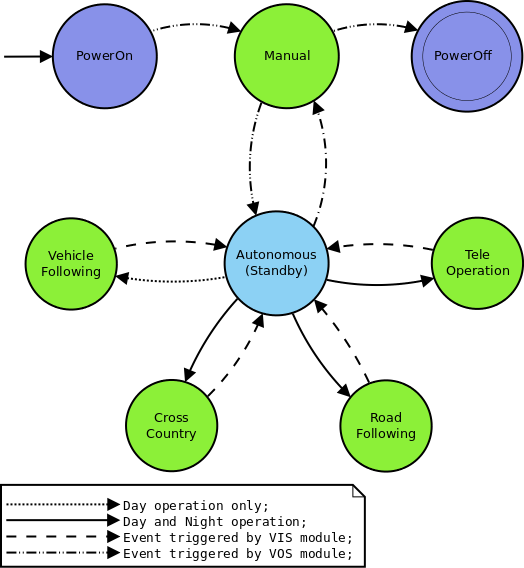
\includegraphics[scale=0.32]{files/VILMA_OPERATIONAL_MODE.png}
	\caption{Modos de operação e troca entre modos.}
	\label{fig:modos_operacao}
\end{figure}

\subsection{Módulos e componentes do sistema}\label{subsec:system_modules_components}

O projeto VILMA é composto por seis sistemas principais (também chamados de módulos), que são: Vehicle Control System (VCS), Vehicle Positioning System (VPS), Vehicle Guidance System (VGS), Vehicle Drive System (VDS), Vehicle Operation System (VOS) e Vehicle Integrity System (VIS). Onde cada sistema possui componentes que realizam tarefas específicas. Os módulos e alguns dos principais componentes presentes na arquitetura do Veículo estão representados na Figura \ref{fig:componentes_sistema}.

\begin{figure}[!ht]
	\centering
	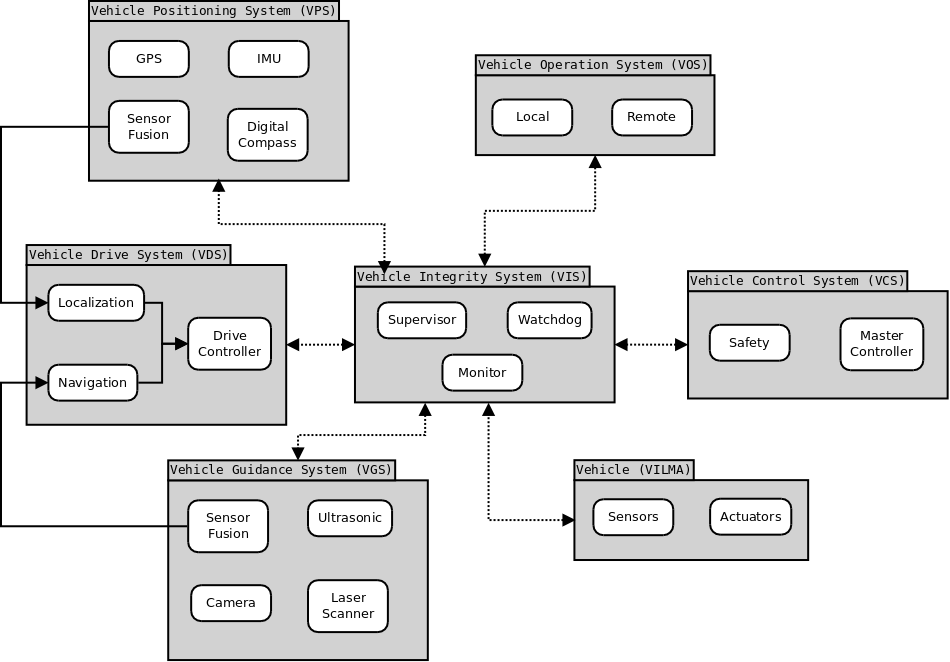
\includegraphics[scale=0.30]{files/VILMA_MODULES_COMPONENTS.png}
	\caption{Módulos e componentes do projeto VILMA.}
	\label{fig:componentes_sistema}
\end{figure}

\subsubsection{Vehicle Driver System}\label{subsec:vds}

O  módulo VCS é responsável por controlar a atuação do Veículo e garantir a segurança dos agentes envolvidos no ambiente de operação. O sistema VCS é responsável por controlar a atuação e garantir a segurança dos agentes envolvidos no ambiente. Sua principal função é fornecer comandos para o controle de velocidade e direção do Veículo, o VCS gera sinais de baixo nível que acionam o sistema mecânico informando a velocidade desejada e a angulação da direção. Ele possui um feedback cíclico para garantir que a velocidade e os comandos de direção estão sendo executados corretamente, levando em conta fatores ambientais, como a derrapagem das rodas.

\subsubsection{Vehicle Integrity System}\label{subsec:vis}


O sistema VIS é responsável por assegurar a integridade dos atores envolvidos no ambiente enquanto o Veículo estiver em funcionamento. Sua principal função é monitorar e coordenar as atividades dos sistemas a fim de obter o comportamento esperado do Veículo.


\subsubsection{Vehicle Position System}\label{subsec:vps}


Assim como o VGS, o sistema VPS possui alguns sensores para realização do posicionamento "global" do Veículo, tais sensores são bussolas, GPS, IMU, etc. As informações recebidas são então processadas e enviadas para que o sistema VDS realize o planejamento da missão.


\subsubsection{Vehicle User System}\label{subsec:vus}

O módulo VOS possibilita a interação do condutor com o automóvel, tanto em modo físico, fornecendo
também o estado do Veículo em tempo real, como alertas e diagnósticos de depuração durante a fase de desenvolvimento. Quanto em modo tele-operado, através da utilização de câmeras instaladas no Veículo para simular a visão do condutor. O operador controla a movimentação do automóvel através de um joystick. 


\subsubsection{Vehicle Guidance System}\label{subsec:vgs}

O sistema VGS utiliza diversos sensores, tais como, scanner laser, câmeras, sensores ultrassônicos para construir mapas digitais do ambiente em torno do Veículo. Os sensores toram o Veículo capaz de reconhecer varias característica do ambiente, tais como estradas, áreas transitáveis, símbolos, etc. também fornece um mapa digital para o VDS que realiza planejamento de trajetória e geração de comandos movimentação ao VCS.

\subsubsection{Vehicle Navigation System}\label{subsec:vns}

O sistema VDS é responsável pela navegação do Veículo afim de alcançar local alvo. Ele deve realizar o planejamento da trajetória até a localização desejada para o Veículo, calcular a velocidade e direção gerando as informações necessárias para que o VCS execute suas tarefas de forma segura. também
monitora a posição do Veículo bem como a execução das manobras a serem realizadas até seu destino.

\subsection{Estados e transições do sistema}\label{subsec:states_transitions}

Para uma adequada coordenação das atividades executadas pelos sistemas do Veículo, é necessário que os componentes possuam um comportamento uniforme em relação ao VIS. Sendo assim, cada componente precisa implementar uma interface comum representada por um conjunto de estados e transições reconhecidos pelo sistema de supervisão possibilitando o gerenciamento das atividades executadas.

Sob a perspectiva do controle supervisório, os estados presentes no sistema são: \textit{PowerOn}, \textit{PowerOff}, \textit{Standby}, \textit{Ready}, \textit{Working}, \textit{Error}, \textit{Emergency}, e \textit{Shutdown}. Cada componente deve conter obrigatoriamente esses estados. Assim, para um dado componente, o significado dos estado e o comportamento geral do Veículo pode ser resumido da seguinte maneira.

Em \textit{PowerOn}

Em \textit{PowerOff}, nenhum sinal elétrico é fornecido ao componente. Em \textit{Standby}, o componente passa a estar energizado, o Veículo continua parado e com o motor ainda desligado. Nesse estado, o sistema não está vinculado a um modo de operação, ao aguardo pela escolha do usuário.

Em \textit{Ready}, o componente está vinculado a um modo de operação mas ainda não está operado nesse modo, o Veículo continua estacionado, porém com o moto em funcionamento. O motivo pela separação entre estes dois estados deve-se ao fato deste trabalho se concentra no comportamento geral do Veículo, sendo a razão devido a necessidade de uma clara separação temporal entre os estados onde o Veículo possa ser comutado para modo de operação manual e o estado onde o Veículo está preparado para operar em modo autônomo. 

Essa separação temporal dos estados é necessária para à sincronização das atividades dos componentes antes que eles entrem no estado \textit{Working}.

Uma vez no estado \textit{Working}, o componente está operando em um dos modos permitidos e o Veículo está em movimento.

Em \textit{Error} e \textit{Emergency}, o componente executa tarefas relevantes a manipulação de exceções ou respostas de emergência.

Em \textit{Shutdown}, o componente deve executar um conjunto predefinido de rotinas que preparam o Veículo para ser desligado.

Todos componentes, inclusive o componente VIS devem possuir os estados citados anteriormente.

As transições entre os estados consistem em um conjunto de atividades que levam os componentes de um estado a outro. Para uma transição ocorrer, ela deve ser disparada por um evento, uma vez disparada as atividades associadas à transição devem ser realizadas com sucesso para que o componente entre em novo estado. O diagrama do estados e suas transições pode ser visto na Figura \ref{fig:estados_transicoes}.

\begin{figure}[!ht]
	\centering
	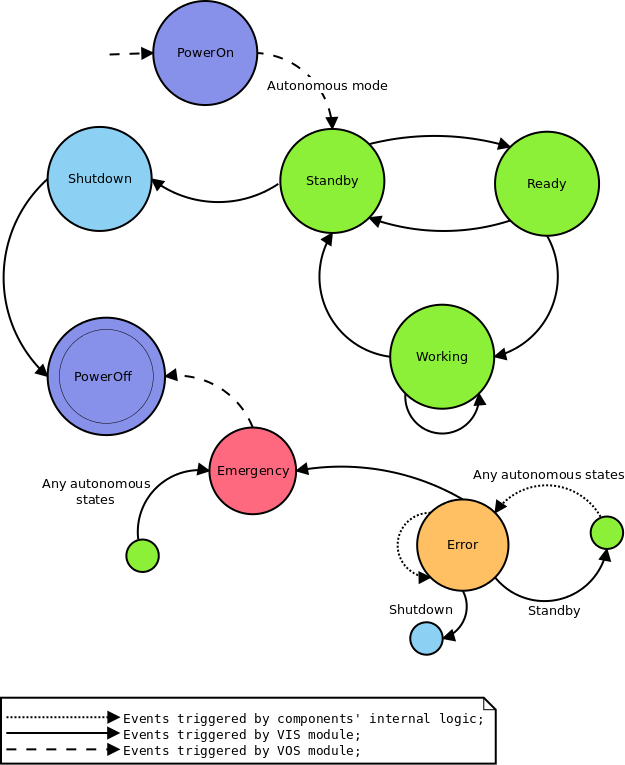
\includegraphics[scale=0.32]{files/VILMA_STATE_MACHINE2.png}
	\caption{Estados e transições dos componentes.}
	\label{fig:estados_transicoes}
\end{figure}

Embora cada componente contenha o conjunto de estados e transições obrigatórios, a questão sobre as atividades envolvidas nos estados e transições é transparente para o VIS. Em outras palavras, o VIS não conhece internamente a complexidade das tarefas executadas dentro dos estados ou durante as transições de um componente e não existe restrição que ele possua apenas estes estados e transições. As atividades envolvidas nas transições de cada componente podem ser diferentes daquelas presentes em outros componentes.

\subsection{Proposta de implementação}\label{subsec:proposal_implementation}

A estrutura de estados e transições apresentada pela Figura \ref{fig:estados_transicoes} precisa ser implementada em cada componente e no VIS como um processo de software. O VIS interage com os outros componentes com base nesta estrutura para realizar a supervisão das atividades do Veículo. não existe uma interação ponto a ponto entre os componentes para o gerenciamento desta interface. A estrutura de estados e transições, como mostrado na Figura \ref{fig:estados_transicoes}, define o comportamento dos componentes reconhecíveis pelo VIS. Entretanto, não existe nenhuma restrição para que os componentes possuam estados e transições próprias necessários para que executem suas atividades corretamente. Um componente pode possuir quantos estados e transições forem necessárias, a única diferença entre os estados e transições adicionais é que esses não serão reconhecidos pelo VIS.
% respeitar o determinismo

Por exemplo considere o componente responsável pela navegação do automóvel (\textit{Planning}). O estado \textit{Working} do \textit{Planning} pode ser dividido em um subconjunto contendo subestados, por exemplo, \textit{Working-cross-country}, \textit{Working-teleoperation}, etc. Estes subestados certamente vão possuir diferentes conjuntos de tarefas. Em particular, no subestado \textit{Working-teleoperation}, o \textit{Planning} pode não possuir nenhuma tarefa específica, ou seja, uma transição "vazia". No entanto, quando o VIS requisitar que todos os componentes realizem a transição para o estado \textit{Working} com o Veículo operando no modo \textit{Teleoperation}, o componente \textit{Planning} vai move-se para esse estado, embora internamente para o \textit{Planning} esta transição possa ser indiferente quanto a transição partindo do estado \textit{Standby}.

Ao adotar o diagrama de estados e transições apresentado pela Figura \ref{fig:estados_transicoes} como uma interface padrão de comportamento entre o VIS e os demais componentes, as atividades internas destes componentes tornam-se transparentes para o sistema de supervisão. Isso garante o gerenciamento das atividades sem que o VIS precise interferir na estrutura e operações individuais de cada componente.

\subsubsection{Comportamento dos componentes}\label{subsec:comportamento_componentes}

% Novo estado PowerOn
Após ser inicializado o sistema, cada componente deve realizar seu processo de inicialização, então, caso o operador tenha ativado o modo de operação do Veículo para autônomo, os VIS deve solicitar que os demais componentes realizem seu procedimento de transição para o estado \textit{Standby} e aguardem novas instruções do sistema supervisório. Uma vez em \textit{Standby}, o VIS pode instruir os componentes para o estado \textit{Shutdown}, caso de falha em algum componente, ou se prepararem para um modo de operação específico Os componentes poderão mover-se para o estado \textit{Ready} caso tenham realizado seus processos inicialização que garantam sua ativação ao modo de operação especificado, conforme instruções do VIS. Assim que o processo seja cumprido, o VIS pode instruir aos componentes que comecem a operar, levando-os ao estado \textit{Working}. Estando neste estado, o VIS pode instruir que os componentes possam retornar ao o estado \textit{Standby}, em caso seja necessária a troca do modo de operação.

Erros operacionais podem ocorre quando um componente está em qualquer dos seguintes estados: \textit{Standby}, \textit{Ready} e \textit{Working}. Cabe exclusivamente ao componente decidir o que constitui uma exceção. Quando alguma exceção ocorrer, o VIS pode instruir o componente em questão tanto para que realize uma reinicialização ou seu desligamento. Caso seja reiniciado, o componente será levado ao estado \textit{Standby}.

Uma emergência pode ocorrer quando um componente está em algum dos seguintes estados: \textit{Standby}, \textit{Ready}, \textit{Working } ou \textit{Error}. O supervisório responderá a uma emergência por duas formas, de acordo com a gravidade do ocorrido ou de reagindo a decisão do operador, que pode instruir o componente a ser reiniciado e colocado em estado de \textit{Standby} após a emergência ser solucionada, ou optar pelo desligamento do componente.



\subsection{Formalização do modelo proposto}\label{subsec:formal_synthesis}

LER ARTIGOS TÉCNICAS DE CONTROLE PARA EVENTOS DISCRETOS

Tendo modelado o comportamento de cada componente em termos de estados e transições, é possível formalizar a lógica do projeto VIS através de técnicas teóricas mais avançadas Uma das possíveis técnicas a teoria de controle para sistemas supervisórios de evento discreto \cite{Event_Systems}. A aplicação desta técnica exige que os estados e transições dos componentes sejam expressos em conjuntos de autômatos (chamados de modelos), enquanto o comportamento desejado do Veículo seja expresso por outro conjuntos de autômatos (chamados especificações). Por exemplo, o comportamento de um componente, seguindo as especificações do VIS como ilustrado na Figura \ref{fig:estados_transicoes}, pode ser representado por um automato $G = (Q,\Sigma,\delta,q_{0},Q_{m})$, onde $Q$ é um conjunto de estados, exemplo, $Q =$ \{\textit{Power-off, Standby, Ready, Working, Exception, Emergency, Shutdown}\}, $\Sigma$ é um conjunto de transições, exemplo, $\Sigma =$ \{\textit{1,2,3,4, 5,6,7,A,B,C,D,E,F,G,H,I,J,K,L,a,p}\}, $\delta$ é a função de transição que especifica o novo estado após a transição do estado atual, como apresentado pela Tabela \ref{tab:func_transicao}, $q_{0}$ é o estado inicial do componente e $Q_{m}$ é o conjunto de estados que indicam a conclusão de determinada sequencia das operações desejadas.

% Please add the following required packages to your document preamble:
% \usepackage{multirow}
\begin{table}[h]
	\centering
	\adjustbox{max height=\dimexpr\textheight-5.5cm\relax, max width=\textwidth}{
		\renewcommand{\arraystretch}{0.75}
		\begin{tabular}{|c|c|c|}
			\hline
			\multicolumn{3}{|c|}{$\delta(old state, transition) = new state$} \\ \hline
			Old state & transition & new state \\ \hline
			power off & 1 & standby \\ \hline
			\multirow{4}{*}{standby} & 2 & ready \\ \cline{2-3} 
			& 6 & shutdown \\ \cline{2-3} 
			& A & exception \\ \cline{2-3} 
			& H & emergency \\ \hline
			\multirow{4}{*}{ready} & 4 & working \\ \cline{2-3} 
			& 3 & standby \\ \cline{2-3} 
			& B & exception \\ \cline{2-3} 
			& I & emergency \\ \hline
			\multirow{3}{*}{working} & 5 & standby \\ \cline{2-3} 
			& C & exception \\ \cline{2-3} 
			& J & emergency \\ \hline
			\multirow{3}{*}{exception} & D & standby \\ \cline{2-3} 
			& E & shutdown \\ \cline{2-3} 
			& $\alpha$ & exception \\ \hline
			\multirow{3}{*}{emergency} & H & standby \\ \cline{2-3} 
			& L & power-off \\ \cline{2-3} 
			& $\beta$ & emergency \\ \hline
			shutdown & 7 & power-off \\ \hline
		\end{tabular}
		\renewcommand{\arraystretch}{1}
	}
	\caption{função de transição $\delta$.}
	\label{tab:func_transicao}
\end{table}

Uma vez que cada componente do sistema é modelado por um automato $G_{i}$, um modelo composto sobre o comportamento geral do Veículo pode ser construído

utilizando o procedimento chamado \textit{"synchronous product"}, representado pelo símbolo $\lvert$ \cite{Event_Systems_ebook}. O resultado em fornecer o produto

síncrono sobre todo $G_{i}$ é um novo automato que representa o comportamento "livre" (não controlado), das atividades simultâneas dos componentes. Ou seja, 

$G = G_{1} \lvert G_{2} \lvert G_{3} \lvert ... \lvert G_{n}$.  

O comportamento esperado para o Veículo pode ser então imposto ao comportamento "livre" a fim de se obter as estratégias de controle de supervisão esperadas pelo VIS. Formalmente, tal comportamento desejado também é expresso em autômatos, chamados de especificações. Ao impor as especificações do modelo composto do Veículo, um conjunto de sequencias de transições pode ser obtido, onde, quando executado pelo VIS garantirá que o comportamento do Veículo atenderá as especificações enquanto o controle exercido pelo VIS for "minimamente restritivo".

Ao utilizar esta abordagem, é possível sintetizar as estratégias de controle de supervisão que permitam que o Veículo lidar com várias situações distintas. Por exemplo, suponha que devido a considerações de temporização, o VCM só possa entrar no estado \textit{Working} após o VAM estiver no estado \textit{Working}. Isso pode ser considerado como um dos requisitos que constituem o comportamento desejado. Esse requisito pode ser expresso como uma especificação $S_{i}$, como apresentado na Figura \ref{fig:exemplo_especificacao}, onde os auto laços representam outras possíveis transições que podem ocorrer no sistema.


\begin{figure}[h]
	\centering
	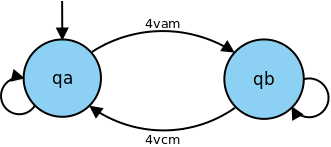
\includegraphics[scale=0.4]{files/VILMA_TRANSITION_EXAMPLE.png}
	\caption{Exemplo de uma especificação, $4_{vam}$: Transição do estado \textit{Ready} para \textit{Working} no componente \textit{Vehicle Actuation}, $4_{vcm}$: Transição do estado \textit{Ready} para \textit{Working} no componente \textit{Vehicle Control}.  }
	\label{fig:exemplo_especificacao}
\end{figure}

Um controle supervisório que garanta o comportamento dos componentes, como um todo, satisfaça a especificação imposta por $S_{i}$ pode ser obtido, dentre outras formas, pelo algoritmo chamado SUPCON \cite{wonham1987supremal}. Este algoritmo gera sequencias de eventos sob a forma de outro automato $V$, exemplo, $ V = SUPCON(G,S_{i})$, que possa ser implementado para garantir o comportamento do Veículo.

Ao expressar vários requisitos sobre o comportamento do Veículo em especificações, é possível obter um método sofisticado de controle pode ser desenvolvido que quando implementado pleo VIS vai garantir que o comportamento do Veículo atenderá todos os requisitos impostos pelos componentes. Essa abordagem formal permite o desenvolvimento sistemático de estratégias de controle supervisório corretas. além de permitir a Introdução de "inteligencia programada" sobe o comportamento do Veículo, consequentemente, melhorando seu grau de autonomia.

% -------------------- NEW SECTION -------------------- 
% -------------------- NEW SECTION -------------------- 
% -------------------- NEW SECTION -------------------- 

\section{Especificação das metodologias e ferramentas}\label{sec:specifications_tools}
Para cumprir com os critérios determinísticos de um sistema crítico de tempo real, é necessário que haja um sofisticado ambiente de hardware e software. Porém, este trabalho concentra seus esforços em prover uma arquitetura inicial com foco em tecnologias e metodologias baseadas puramente em softwares capazes de realizar tarefas em tempo real rígido.

Antes de descrever as especificações do sistema de controle supervisório, será apresentado brevemente alguns conceitos para uma melhor compreensão do tipo de ambiente escolhido com o intuito de atender aos requisitos necessários para a realização deste projeto.

Vale ressaltar que a metodologia de escolha para a proposta da arquitetura a ser desenvolvida baseia-se nos estudos e resultados previamente realizados por outros pesquisadores, não sendo considerada uma escolha definitiva.

\subsection{Sistemas críticos}\label{subsec:critical_systems}

Um sistema é chamado em tempo real crítico se uma determinada tarefa deva ser concluída antes que um determinado valor de tempo seja atingido. As consequências causadas caso esse intervalo de tempo seja excedido, classificam o sistema, na maior parte dos casos, em duas categorias \cite{Sticha_BMW_ROS}:

\begin{itemize}
	\item \textit{\textbf{Hard}} o tempo limite não pode ser excedido em nenhuma circunstância, pois caso ocorra leva a uma falha total do sistema. 
	
	Algumas das principais exigências dos sistemas essa categoria são: latência mínima durante a alternância de tarefas, \textit{jitter} mínimo, gerencia da tarefa até sua conclusão, multitarefas preemptivas, herança de prioridades e atender rigorosamente aos tempos de resposta e execução determinados.
	
	Como exemplo, o sistema de freios do Veículo. Se ele demorar muito tempo para responder, o Veículo pode bater e causar um acidente.
	
	\item \textit{\textbf{Soft}} atender aos prazos determinados é importante, mas a falha em alguns deles não é catastrófica ao sistema e o resultado pode ser utilizado após o período excedido, porém, a qualidade do resultado obtido é reduzida.
	
	Como exemplo, uma aplicação que utiliza \textit{streaming} de vídeo. Se os dados de vídeo chegam muito lentamente ao usuário, o vídeo consequentemente vai ficar pausado por algum tempo durante o carregamento do vídeo, o que implica na diminuição da qualidade. 
	
	No entanto, mesmo que houver falha na transmissão e dados forem perdidos, a reprodução do vídeo poderá continuar a ser exibida.
\end{itemize}

além disso, é importante entender a diferença entre sistemas de tempo real e performance. O único objetivo da otimização e performance em sistemas é obter uma resposta média tão rápida quanto for possível. Raros valores de pico são aceitáveis, desde que suas ocorrências não sejam suficientes para influenciar no desempenho médio do sistema.

Sistemas de tempo real tem objetivo diferente. Aqui o tempo médio de resposta não é importante, e sim os valores de pico que ocorrerem. Como mencionado anteriormente, em sistemas com requisitos de tempo real rígido um único valor de pico que ocorra e exceda o prazo (deadline) determinado causa a total falha no sistema. Portanto, a característica importante dos sistemas de tempo real não é a sua performance média, mas sim seu comportamento determinístico. 

Mesmo que uma determinada tarefa seja realizada com maior velocidade, em média, por um sistema de alto desempenho sem propriedades em tempo real, a sua falta de comportamento determinístico torna impossível garantir o máximo tempo de resposta.

\subsubsection{Real-Time X Fast-Time}

\subsection{Sistema Operacional Linux}\label{subsec:so_linux}

Linux é um dos sistemas operacionais mais difundidos entre a comunidade cientifica e industrial, possui distribuições para uma série de plataformas diferentes. Em sua versão padrão o \textit{kernel} Linux permite apenas que um processo execute seu código por vez se determinadas condições forem respeitadas \cite{build_xenobuntu}. 

Isso leva ao cenário em quem um processo de alta prioridade demande que a CPU precise esperar por vários milissegundos, por exemplo, para que o código do \textit{kernel} complete sua execução até que o \textit{scheduler} garanta sua requisição.

Embora isto seja aceitável em alguns ambientes, a latência introduzida certamente levará a falha total em sistemas críticos de tempo real. 

Para resolver esse problema foram criadas algumas abordagens que são aplicadas ao \textit{kernel} Linux, entre as mais difundidas estão as denominadas \textit{Micro-kernel} e \textit{Nano-kernel}.

A ideia básica em transformar o \textit{kernel} padrão do Linux em um sistema tempo real extremamente rígido é ter um \textit{kernel} de alta prioridade sendo executado entre o \textit{hardware} e o Linux, onde as tarefas de tempo real são executadas por este \textit{kernel} sem interrupção e os processos normais ficam completamente suspensos durante este período.

O escalonador do \textit{kernel} de tempo real trata o \textit{kernel} padrão como uma tarefa ociosa, onde, se nenhuma tarefa de tempo real estiver sendo executada o \textit{kernel} padrão pode executar seu próprio escalonador para agendar seus processos.

Entre as implementações mais difundidas estão o RTAI e Xenomai que são conceitualmente homogêneos, ambos utilizam o \textit{kernel} Linux de propósito geral e a API de tempo real.
Para lidar com as interrupções, ambos RTAI e Xenomai utilizam \textit{Adaptive Domain Environment for Operating Systems} (ADEOS). As interrupções de \textit{hardware} são interceptados pelo ADEOS e encaminhadas logicamente através da estrutura de \textit{pipe} para outros componentes, como Linux, RTAI, ou Xenomai \cite{ADEOS}.

Entretanto, existe uma diferença sutil na forma com que eles manipulam as interrupções de \textit{hardware}. A abordagem utilizada pelo RTAI (Figura \ref{fig:rtai}) pode lidar com as interrupções não apenas usando ADEOS mas também por interceptações. Ao contrario do Xenomai (Figura \ref{fig:xenomai}) que manipula todas as interrupções utilizando o ADEOS.

\subsubsection{Comparação RTOS}

\subsection{Xenomai}\label{subsec:xenomai}

Xenomai é baseado no \textit{framework} ADEOS, capaz de proporcionar um ambiente flexível para o compartilhamento dos recursos de \textit{hardware} entre vários sistemas operacionais ou entre várias instâncias de um único sistema operacional \cite{ADEOS}. Para tornar possível a execução na mesma plataforma entre múltiplos \textit{kernels} em paralelo de maneira segura, ADEOS possui um compartilhamento eficiente dos recursos críticos de \textit{hardware}, permitindo estabelecer prioridades para cada domínio, ou seja, cada SO em execução. 

A estrutura original foi criada para ser uma camada de virtualização de máquinas em ambientes de computação distribuída. Em sua versão simplificada, conhecida como I-Pipe (\textit{Interrupt Pipeline}), o projeto foi alterado para atender à latências determinísticas no gerenciamento de interrupções, o que é fundamental para operações em tempo real.

Xenomai possui um conjunto de componentes principais que fornecem funcionalidades básicas para operações de tempo real, que atuam como um \textit{nano-kernel}, ou seja, ele depende do \textit{kernel} do Linux para executar as tarefas que não estejam no escopo determinístico.

Xenomai inclui alguns componentes adicionais, que fornece funções como base para as operações em tempo real, que atua como um \textit{nano-kernel}, ou seja, ele depende do \textit{kernel} do Linux para tudo que não é capaz de fazer por si só. Os principais componentes e funcionalidades de Xenomai são descritos a seguir.

\begin{itemize}
	\item \textbf{Nucleus} é o núcleo do RTOS, sendo responsável pela criação de \textit{threads}, agendamento de processos, sincronização, alocação de memória e gerenciamento de interrupções \cite{Silberschatz:2001:OSC:559069}.
	
	\item \textbf{RTDM} o \textit{Real-Time Driver Model} (RTDM) é uma estrutura para o controlador do projeto de tempo real, arquivos, \textit{socket I/O} e a descrição de manipulação \cite{Kiszka}. 
	
	\item \textbf{High resolution timers} outro recurso importante do Xenomai é o suporte para temporizadores de alta resolução, que possuem precisão de microssegundos para agendamento de eventos \cite{Bhaira_linux_xenomai_pcidata}.
	
	\item \textbf{Skins} são camadas emuladas de outros RTOS existentes, como VxWorks, pSOS+, VRTX, RTAI, uITRON \cite{barr2003choosing}.
\end{itemize}

O projeto padrão das \textit{skins} do Xenomai é uma API com as seguintes característica:

\begin{itemize}
	\item \textbf{Real-time IPC} é um conjunto completo de \textit{Inter-Process Communication} (IPC), entre outros recursos, ele possui suporte a filas de mensagens, passagem de mensagens um-para-um e \textit{pipes} que fornecem um canal de comunicação livre de latência entre as tarefas em tempo real e processos padrões \cite{barabanov1997linux}. 
	
	\item \textbf{Synchronization} a maior parte dos objetos de sincronização clássicos estão implementados dentro das \textit{skins} nativas, tais como, \textit{Mutexes}, \textit{Counting Semaphores}, \textit{Event flags} e \textit{Condition Variables} \cite{Silberschatz:2001:OSC:559069}. 
	
	\item \textbf{Memory} quando é necessária a alocação dinâmica de memória para as tarefas de tempo real, Xenomai usa uma região de memória cujo tamanho é estipulado durante sua inicialização. A atribuição ocorre de forma limitada em tempo, e pode ser utilizada para mapear objetos de memória compartilhada entre \textit{kernels} e do espaço de usuário \cite{Xenomai_API}. 
\end{itemize}

\subsubsection{Típicas operações inseguras em sistemas RT}\label{subsubsec:unsecure_operations_rtos}

Qualquer operação que possa bloquear a aplicação por um intervalo indefinido de tempo é um exemplo de operação que quebra o determinismo do sistema, ex. acessar um dispositivo indisponível, utilizar o canal de envio/recebimento de dados padrão ou alocação/desalocação de memoria na pilha de tarefas. Em resumo, qualquer tipo de instrução com intervalo indeterminado de tempo resulta em uma falha de determinismo.

Sistemas RTOS possuem mecanismos com garantias de tempo real para chamadas do sistema, diferentemente dos sistemas operacionais de propósito geral, porém é necessário checar a documentação especifica do RTOS em uso. Por exemplo, aplicações Xenomai qualquer chamada que realize consultas em uma thread possui garantias de tempo real, porem uma chamada de função sleep é sempre de não tempo real. Ou ainda uma operação que realize um reescalonamento não possui garantias de ser de tempo real.    

Tipicamente alguns recursos das linguagens de programação devem ser utilizados cuidadosamente. Por exemplo, um contêiner vetor da biblioteca C++ STL não possui garantias de tempo real, uma vez que seu tamanho é dinâmico e o SO precisa fazer uma nova chamada de sistema para alocação da quantidade de memoria necessária.

Quando uma tarefa de tempo real ultrapassa seu intervalo de execução, isso incorre em uma estado chamado Overrun. A consequência de um Overrun depende exclusivamente do sistema operacional sendo utilizado, que podem ser tanto invocar um sinal de falha ou a finalização completa da aplicação. 

\subsection{Ethernet}\label{subsec:ethernet}

O protocolo de comunicação \textit{Ethernet} utiliza o método de acesso conhecido como \textit{Carrier Sense Multiple Access/Collision Detection} (CSMA/CD) para proporcionar uma média compartilhada entre computadores. Neste sistema, cada computador detecta o \textit{carrier} ou "escuta" o meio compartilhado para verificar se a rede está sendo utilizada por outro sistema.	Assim, um sistema só pode transmitir caso a rede esteja ociosa, ou seja, não estiver sendo utilizada por outro sistema. Isso garante que nenhum dos sistemas utilize a rede compartilhada após o início da transmissão por outro sistema \cite{Spurgeon:2000:EDG:336070}.

Quando dois ou mais sistemas tentam utilizar a rede para transmitir dados ao mesmo tempo acontece a chamada colisão de pacotes, então o estratégia implementada pelo \textit{Collision Detection} (CD) é executada. CD detecta colisão na rede após a transmissão de um pacote realizada por um computador, através da escuta da rede para verificar se há colisões ao pacote transmitido.

No caso de não haver nenhuma colisão, é dito que a transmissão ocorreu com sucesso. No caso de uma colisão, o computador para imediatamente a transmissão e transmite uma sequência de dados, chamada de \textit{jam}, de 32-bits. A sequencia \textit{jam} garante que qualquer outro nó, que pode nesse momento receber este \textit{frame}, vai receber o sinal \textit{jam} no lugar do MAC 32-bits CRC correto, e descarta o \textit{frame}. Os \textit{frames} de todos os sistemas envolvidos na colisão precisam ser reenviados, uma vez eles foram descartados na colisão. Assim, cada um dos computador fica "ocioso" por uma um período aleatório e retransmite o pacote novamente.

Esse processo é executado constantemente até que cada um dos pacotes seja transmitido com sucesso. O período de tempo "ocioso" é randômico e baseado na equação ($r \times 51.2s$) , onde $r$ é um número aleatório entre $0$ é $2^{10}-1$.

O padrão \textit{Ethernet} tem sido o método de compartilhamento de média mais aceito por muitas razões. Atualmente é um dos meios mais baratos de proporcionar um meio compartilhado de dados entre computadores, seu custo de instalação inclui a criação de placas NIC e conectores em computadores, \textit{Hubs}, \textit{switches} e cabos. além disso, proporciona a flexibilidade de operar em várias taxas de transmissão. Sua ampla aceitação trouxe grande disponibilidade de \textit{hardware} e suporte, simplificando sua utilização, instalação e configuração, o que a tornou um recurso padrão nos sistemas informatizados dos dias atuais.

Porém, existem alguns problemas que precisam ser resolvidos quando se deseja garantir o comportamento determinístico para sistemas distribuídos de tempo real. A \textit{Ethernet\textsl{}} foi projetada para fornecer uma solução simples para utilização de dados compartilhadas, e durante as transmissões ocorrem muitas colisões entre pacotes. As retransmissões trazem aleatoriedade no tempo de transmissão para o comportamento da rede, já que cada sistema envolvido na colisão fica "ocioso" por um período de tempo aleatório. Este atraso devido às colisões e retransmissão pode ser negligenciado em um cenário normal, onde a carga na rede é baixa. No entanto, quando a carga sobre o meio compartilhado é elevada, então o tempo de atraso das mensagens aumenta ainda mais, devido a um maior número de colisões.

aplicações em tempo real exigem qualidade previsível do serviço. Assim, o modelo não-determinístico de \textit{Ethernet}, juntamente com o aumento do tempo de atraso, o torna impróprio sua utilização em um sistema distribuído em tempo real.

A fim de garantir os recursos da \textit{Ethernet} em aplicações de tempo real, é preciso tornar seu comportamento determinístico. Existem abordagens que foram formuladas para resolver este problema. Estas sugestáes podem ser basicamente divididas em duas categorias: soluções de \textit{hardware} e baseadas em \textit{software}. Soluções de \textit{hardware} como \textit{SCRAMNet} e \textit{Token Ring Protocol} possibilitam capacidades de tempo real a rede alterando o \textit{hardware} dos sistemas e possuem melhores resultados. Soluções de \textit{software} como \textit{RTnet} e \textit{Rether} tentam obter o comportamento determinístico de tempo real por modificações do sistema operacional e sem a necessidade de alteração no \textit{hardware}, oferecendo uma solução mais econômica e de maior flexibilidade \cite{Sampathkumar2002}. 	

Esse trabalho tem como objetivo utilizar a solução baseada em \textit{software} através do \textit{framework} RTnet que implementa o método conhecido como \textit{Time Division Multiplexing} sobre o padrão \textit{Ethernet}. Como o nome sugere, esse método realiza a multiplexação de diferentes sistemas na utilização da LAN com base no tempo, onde é atribuído um valor de intervalo de tempo para que cada computador presente na rede possa transmitir um pacote. Como resultado, a qualquer instante, apenas um nó poderá transmitir, evitando as colisões e consequentemente as retransmissões, obtendo comportamento determinístico para a rede \cite{rt_net_IEEE_so53551}.  

O desempenho deste método pode ser pior do que a \textit{Ethernet} baseada em CSMA/CD quando temos um único nó transmitindo uma grande quantidade de dados devido ao fato de que o sistema de transmissão não poder utilizar outros intervalos de tempo, mesmo que a rede não seja utilizada por nenhum outro computador. No entanto, este método garante uma largura de banda fixa e o desempenho não cai abaixo da largura de banda garantida, mesmo quando todos os sistemas na rede estão transmitindo uma grande quantidade de dados.

\subsection{Real-time Ethernet (RTnet)}\label{subsec:rtnet}

Com o objetivo de fornecer uma plataforma de comunicação de tempo real, flexível e independente do \textit{hardware}, o projeto RTnet foi criado em 2001 na Universidade de Hannover. RTnet é uma estrutura puramente baseada em \textit{software} para a troca de dados arbitrários sob rígidas restrições de tempo real. Sua implementação é fundamentada para o SO Linux utilizando as extensões de tempo real RTAI e Xenomai \cite{xenomai_rtnet}. 	%http://www.rtnet.org/download/RTnet-ETFA05.pdf

O projeto da pilha RTnet, como apresentado na Figura \ref{fig:rtnetstack}, foi inspirado na estrutura modularizada do subsistema de rede do Linux. Destinando-se a escalabilidade e capacidade de expansão, a fim de obter diferentes requisitos de aplicação.

\begin{figure}[h]
	\centering
	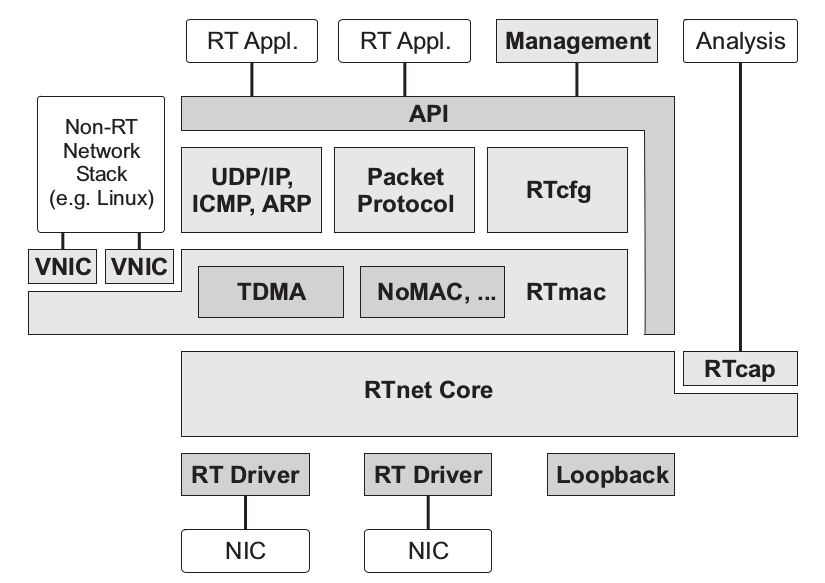
\includegraphics[scale=0.22]{files/rtnet_stack.png}
	\caption{RTnet stack.  \cite{rtnet_org}}
	\label{fig:rtnetstack}
\end{figure}

A RTnet explora a extensão do \textit{kernel} tempo real para assegurar o determinismo na pilha de comunicação. Assim, todas as instruções relacionadas com esse protocolo faz o uso das funções do \textit{kernel} em tempo real, ao invés do \textit{kernel} padrão, que vincula as latências para os tempos de execução nas latências de interrupções possibilitando a comunicação determinística. A Figura \ref{fig:rtnetnetwork} apresenta um modelo básico da integração da RTnet em uma rede.

\begin{figure}[h]
	\centering
	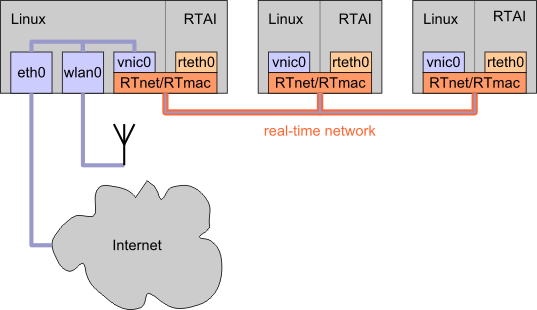
\includegraphics[scale=0.33]{files/rtnet_network.png}
	\caption{RTnet network.  \cite{rtnet_org}}
	\label{fig:rtnetnetwork}
\end{figure}

Sua estrutura é composta por um conjunto de serviços centrais, que rodam entre a camada \textit{Ethernet} e a camada de aplicação (ou camada IP), necessários para a maioria cenário de sistemas críticos distribuídos. Estes serviços são: \textit{TDMA Operation}, \textit{Syncing}, \textit{Protocol stack}, \textit{Physical Layer}, \textit{Data Link Layer}, \textit{TDMA Layer} e \textit{Network and transport layer} \cite{rt_net_IEEE_so53551}.

%http://www.intechopen.com/books/factory-automation/a-real-time-wireless-communication-system-based-on-802-11-mac

A API implementada consiste em \textit{sockets} POSIX para processos em tempo real no espaço de usuário e módulos do \textit{kernel}, através da interface RTDM. Os principais componentes da RTnet são: o gerenciador da pilha, que fornece a manipulação dos pacotes de entrada, e os \textit{drivers}, que realizam a comunicação com o \textit{hardware}. O gerenciador da pilha é uma tarefa de tempo real com prioridade máxima no sistema, onde é realizada a demultiplexação dos pacotes de entrada e passando suas referencias para os respectivos manipuladores, de acordo com o protocolo que o pacote recebido pertence.

O gerenciador da pilha e os \textit{drivers} do dispositivo utilizam uma estrutura chamada \textit{rtskb} para à troca e armazenamento temporário dos pacotes. Seu uso é semelhante à estrutura \textit{sk\_buff} encontrada na pilha de rede Linux. O tamanho do \textit{buffer} é definido estaticamente para a rede MTU (Maximum Transmission Unit), e um numero fixo de \textit{buffers} é alocado e atribuído a cada componente presente a rede durante à inicialização do sistema. Então, cada componente recebe um \textit{rtskb} contendo um pacote e deve retornar um pacote vazio. Assim, no final de cada operação os componentes possuem o mesmo número de \textit{rtskb} \cite{Benvenuti_linux_net}.

RTnet também possui uma camada de \textit{software} intermediário entre UDP/IP e os \textit{drivers}, chamada \textit{RTmac}. Essa camada não é de uso obrigatério, mas é utilizada para alguns serviços úteis fornecidos, por exemplo, a configuração automática (através do módulo \textit{RTcfg}) ou encapsulamento para transmissão de dados em processos de não tempo real utilizando interfaces virtuais. além disso, pode ser definido um mecanismo de acesso ao meio através do \textit{RTmac}, para garantir transmissões livres de colisões e limitadas por tempos determinados. Esses mecanismos são chamados \textit{disciplines}, e podem ser carregados/descarregados dinamicamente. O esquema flexível TDMA possui uma abordagem \textit{master/slave} estática. Ele fornece a sincronização entre o \textit{clock} dos componentes, múltiplas atribuições de \textit{slots} e prioridades de transmissão estáticas. Sua estrutura foi projetada para operações em redes cabeadas e possui um mecanismos de calibração a fino que atenua os efeitos negativos para \textit{jitter} da transmissão.

A abordagem \textit{master/slave} utilizada pelo TDMA \cite{rt_net_IEEE_so53551} a estação \textit{master} é responsável pela sincronização dos componentes, as estações \textit{slave} podem atuar como sistemas de \textit{backup} compensando casos de falhas da estação \textit{master}. A componente \textit{master} realiza o envio regularmente de um pacote de sincronização aos outros componentes, que marca o início da transmissão de um \textit{frame} TDMA. Cada transmissão de um \textit{frame} é dividida em intervalos de tempo e contem um identificador numérico que é incrementado quando um novo \textit{frame} for iniciado. 

Cada estação pode ter um ou mais \textit{slots} atribuídos para à transmissão, com uma fila separada em pacotes para cada intervalo de tempo. Também é possível atribuir vários \textit{slots} para cada fila de saída. Onde, cada intervalo de tempo pode ser compartilhado entre múltiplas estações, que por sua vez podem utilizá-los. Na Figura \ref{fig:rtnet_tdma} é apresentada uma configuração simples para um ciclo do TDMA. A estação \textit{master} define o tempo do ciclo, enquanto as estações \textit{slave} devem configurar seus \textit{slots} de transmissão corretamente. A configuração pode estar presente em cada estação como um arquivo de texto ou pode ser distribuída pela estação \textit{master} para todas os participantes \textit{slave} antes do início da fase de calibração utilizando o serviço de configuração RTnet, chamado RTcfg. Um intervalo de tempo atribuído a uma estação transmissora deve ser especificado como um \textit{offset} relativo ao \textit{frame} TDMA inicial, isto é, em relação à transmissão do pacote de sincronização enviado pelo \textit{master}.

\subsection{Sistemas robóticos}\label{subsec:robot_systems}

\subsection{Open Robot Control Software (OROCOS)}\label{subsec:orocos}

\textit{Open Software de Controle Robot} (Orocos) é um \textit{framework} de software para o controle de robôs em tempo real, com foco em industrias. É escrito em C++ sob a licença \textit{GNU Lesser GPL} com suporte aplicações que utilizem GNU/Linux, RTAI/LXRT e Xenomai. Seu objetivo é fornecer uma estrutura altamente modular, de fácil integração com outros sistemas robóticos, com foco alta performance, para um avançado controle de robôs e máquina. \cite{Orocos_manual}.

Entre outras, Orocos possui quatro bibliotecas principais \cite{Orocos_Project_IEEE}, que são:

\begin{itemize}
	\item A biblioteca Orocos Real-Time Toolkit (RTT): não é propriamente uma aplicação, sua função dentro do ecossistema do framework é fornecer uma infraestrutura funcional para construir aplicações robóticas em C++. Sua enfase é no desenvolvimento de sistemas críticos, interativos e baseados em componentes.
	\item A biblioteca Orocos Components Library (OCL): provê algumas funções para o controle, gerenciamento e interação dos componentes da aplicação. Alem disso, também existem meios para o acesso ao hardware do sistema em questão.
	\item Orocos Kinematics and Dynamics Library (KDL): é uma biblioteca escrita em C++ que permite o calculo para cadeias de operações cinemáticas em tempo real.
	\item Orocos Bayesian Filtering Library (BFL): é uma aplicação independente com foco em redes dinâmicas Bayesiana, exemplo, algoritmos de processamento de informações e estimativa recursiva baseado na regra de Bayes, tais como Filtros de Kalman Estendido, filtro de partículas (métodos sequenciais de Monte), entre outros
\end{itemize}

Neste trabalho é utilizado apenas as bilbiotecas OCL e RTT. Onde OCL é responsável para a configuração, inicialização e gerenciamento dos componentes desenvolvidos sob a biblioteca RTT. Esta biblioteca permite que os componente \cite{Orocos_manual}:

\begin{itemize}
	\item Lock free, thread-safe, inter-thread function calls.
	\item Communication between hard Real-Time and non Real-Time threads.
	\item Deterministic execution time during communication for the higher priority thread.
	\item Synchronous and asynchronous communication between threads.
	\item Interfaces for component distribution.
	\item C++ class implementations for all the above.
\end{itemize}

A biblioteca Real-Time Toolkit (RTT) permite que os desenvolvedores de aplicações criarem sistemas configuráveis e interativos baseados em componentes de controle em tempo real. Esta biblioteca foi escrita para desenvolver componentes que podem comunicar-se através de processos locais ou distribuídos em rede, além da capacidade de configuração em tempo real através de arquivos XML.

\begin{figure}[h]
	\centering
	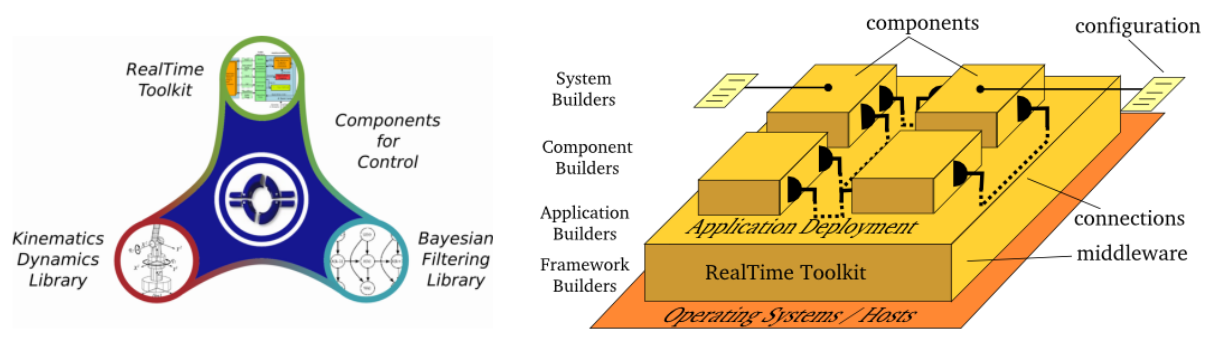
\includegraphics[scale=0.22]{files/orocos_stack.png}
	\caption{Orocos framework.  \cite{Orocos_manual}}
	\label{fig:orocos_stack}
\end{figure}

Uma vez que sistemas Orocos possuem estrutura modular, as aplicações são formadas por componentes de uso específico que podem se comunicar através de uma rede. Seu meio de comunicações padrão é baseado na abordagem CORBA.

A Figura \ref{fig:orocos_app_stack} apresenta a estrutura de uma típica aplicação Orocos-RTT.

\begin{figure}[h]
	\centering
	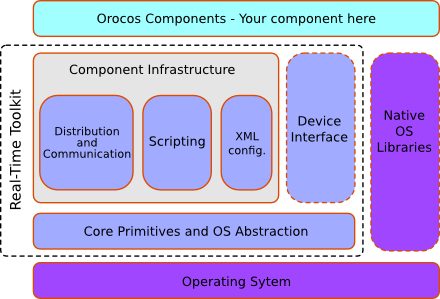
\includegraphics[scale=0.33]{files/ApplicationStack2.png}
	\caption{Estrutura de uma aplicação RTT.}
	\label{fig:orocos_app_stack}
\end{figure}

Um componente é construído herdando a classe TaskContext, que implementa uma tarefa que possui mecanismos de criação de threads seguras e eficientes "portas" para a troca de dados sem a perda do modelo determinístico do sistema. Um componente pode reagir a eventos, comandos de processo, ou executar maquinas de estado em tempo real, entre outras funcionalidades \cite{Orocos_manual}. A Figura \ref{fig:taskcontex} apresenta uma visão geral da classe TaskContext. 

\begin{figure}[h]
	\centering
	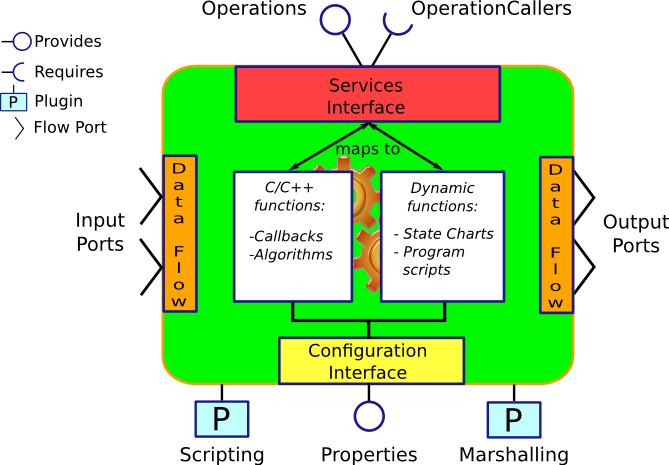
\includegraphics[scale=0.33]{files/ATaskContext.png}
	\caption{Visão geral da classe TaskContex.}
	\label{fig:taskcontex}
\end{figure}

Existem cinco maneiras opcionais de se interligar componentes Orocos, como mostrado na Figura \ref{fig:orocos_network}: através de \textit{properties} (parâmetros que podem ser modificados em tempo de execução), por meio de \textit{events} (funções que executadas quando determinadas mudanças ocorrerem), utilizando \textit{methods} (funções que produzem resultados imediatos), com \textit{commands} (procedimentos para alcançar determinado objetivo) e por \textit{dataflows} (canais de transporte de dados sem \textit{buffer}, utilizando \textit{threads} seguras).

\begin{figure}[h]
	\centering
	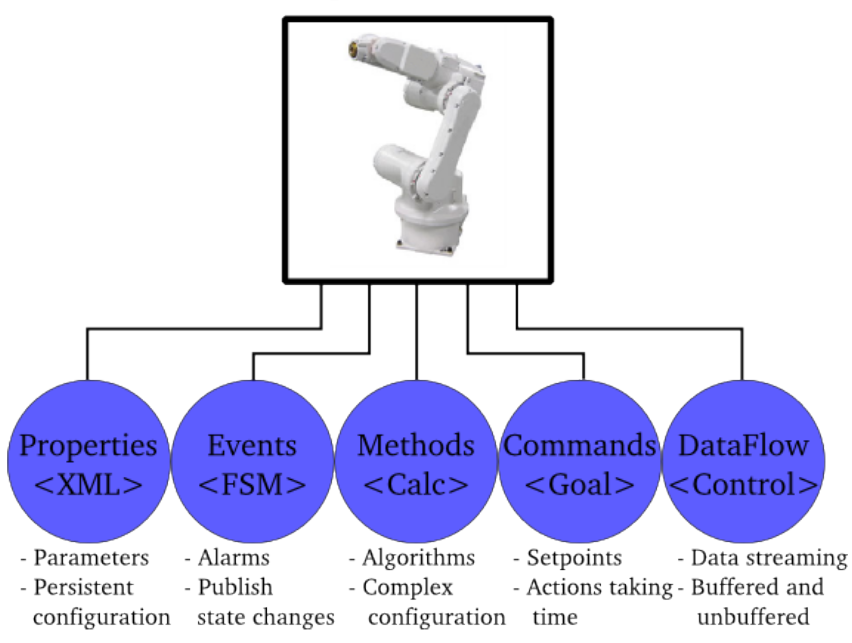
\includegraphics[scale=0.22]{files/orocos_network.png}
	\caption{Orocos interfaces.  \cite{Orocos_manual}}
	\label{fig:orocos_network}
\end{figure}

além de definir os mecanismos de comunicação citados acima, Orocos permite que a aplicação seja formada por máquinas de estados hierárquicos que utilizem essas primitivas nos componentes, esta é a forma que Orocos define a lógica específica da aplicação. As máquinas de estados podem ser ou não carregadas em tempo de execução em um componente \cite{Orocos_Cobem}.

%ros comunication integration.pdf

\subsection{Robot Operating System (ROS)}\label{subsec:ros}

O \textit{Robot Operating System} (ROS) é um meta sistema operacional com o objetivo ao rápido desenvolvimento de \textit{softwares} robóticos, criado pela Willow Garage \cite{willow_ROS}. ROS tornou-se um \textit{framework} muito difundido, provavelmente o mais ativo e adotado no campo de pesquisas, devido ao grande numero de módulos nativos disponíveis, alem dos muitos criados pelas comunidade colaboradora. 	%ros comunication integration.pdf

Seu código fonte é liberado sob a licença BSD revisada, para que ele possa ser livremente modificado e utilizado por amadores e instituições, mas também por empresas comerciais, alguns pacotes são liberados sob licenças mais restritivas, como a GPL.

É executado nativamente no Linux Ubuntu, mas tem algum grau de suporte para outros sistemas operacionais \textit{Unix-like}. As bibliotecas clientes do ROS core são escritas principalmente em C++, Python, e Lisp, com suporte experimental para Java, Lua e Mono/.NET.

Sua arquitetura é altamente modular, \textit{softwares} desenvolvidos com ROS são compostos por um conjunto de nós (chamados Nodes), que são elementos de processamento virtual proporcionando interfaces e operações muito específicas.

Por exemplo, existem \textit{Nodes} para extrair primitivas geométricas de imagens estáreo, outros para o planejamento de tragetória, inteligência artificial, controle de movimento, interfaces para periféricos (por exemplo, \textit{joysticks}, \textit{Microsoft Kinect}, escâneres a laser, servomotores), etc \cite{ros_components}.

\textit{Nodes} por si só tem propósito pequeno, mas, conectando-os, é possível construir uma aplicação robótica muito complexa. Eles se comunicam através da técnica de \textit{publish} e \textit{subscribe}. \textit{Nodes} quem produzem algum tipo de dados os publica através de um tópico de tipo específico, e os nós que precisam desses dados os recebem, assinando a esse tópico, conceito apresentado pela Figura \ref{fig:ros_pubsub}.

\begin{figure}[h]
	\centering
	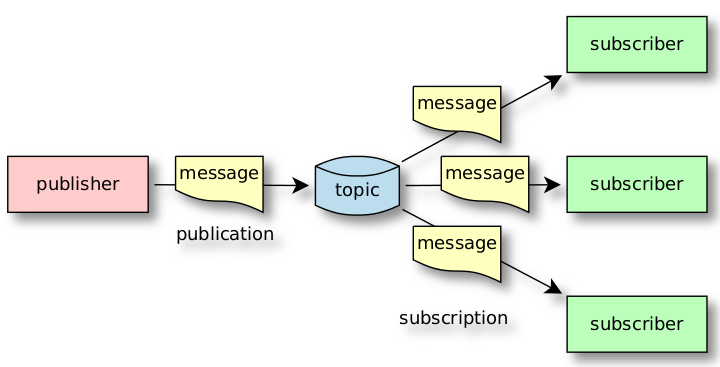
\includegraphics[scale=0.22]{files/ros_pubsub.png}
	\caption{Fluxo conceitual de mensagens para um tópico publicado e subscrito.  \cite{ros_components}}
	\label{fig:ros_pubsub}
\end{figure}

ROS suporta o \textit{streaming} de dados contínuos através de tópicos, a técnica de chamadas \textit{request/response} para serviços globais e o compartilhamento de parâmetros de ambientes. A configuração e controle dos \textit{Nodes} na rede é realizada baseada no protocolo \textit{XML-RPC}, que garante o máximo de portabilidade entre qualquer plataforma que suporta o protocolo \textit{TCP/IP}, existe um nó centralizado, chamado \textit{Master}, que supervisiona toda a rede.

Ao contrário dos \textit{Nodes}, \textit{topic} e \textit{service} de fluxos de dados adotam um protocolo personalizado de baixo nível, que normalmente é baseado em TCP, mas também com base em UDP para aplicações sensíveis à latência \cite{OKa13_ROS_Gentle}.  

Os programas desenvolvidos com ROS podem ser agrupados em pacotes (chamados \textit{packages}) ou pilhas (chamadas \textit{Stacks}). Um pacote de ROS é um formado por um conjunto de códigos que fornece uma funcionalidade específica para ser reutilizado com facilidade. Por exemplo, existem pacotes para um sensor em particular, ou para um algoritmo de localização específico.	Um pacote pode conter ROS Nodes, bibliotecas independentes, conjuntos de dados, arquivos de configuração, ou qualquer coisa que necessária a um módulo.

As pilhas são formadas por conjuntos de pacotes que compartilham um objetivo comum, por exemplo, visão computacional ou planejamento de tragetória. Elas podem ter dependências de outras pilhas, de forma a serem mantidos de forma independente.

Algumas regras definem a estrutura do sistema de arquivos dos \textit{packages} e \textit{stacks}, de modo que eles possam ser compilados de forma automatizada por meio de um conjunto de ferramentas, com base no sistema de construção \textit{CMake}, mantendo o código organizado e sustentável por pessoas diferentes \cite{cmake_org}.

\subsection{Integração entre OROCOS e ROS}\label{subsec:rtt_ros_integration}

A integração entre o \textit{framework} OROCOS e o sistema ROS pode ser realizada, sem complicações, utilizando a biblioteca \textit{rtt\_ros\_integration} \cite{rtt_ros_integration}. Uma breve descrição sobre como essa integração acontece é apresentada a seguir:

\begin{itemize}
	\item \textbf{Data flow} Os componentes de OROCOS possuem estruturas chamadas de \textit{data ports}, meio por onde os componentes trocam dados entre si e os processos. No sistema ROS esse mecanismo é equivalente aos \textit{nodes} , que realizam a troca de informações entre os \textit{topics}. através da biblioteca de integração, componentes OROCOS podem publicar dados para os \textit{topics} do ROS e vice versão.
	
	\item \textbf{Properties} Componentes OROCOS também possuem variáveis chamadas \textit{property}, ao passo que \textit{nodes} em ROS possuem os chamados \textit{parameters}. Assim, a biblioteca torna possível que os componentes OROCOS leiam os parâmetros oriundos dos \textit{server parameter} em ROS.
	
	\item \textbf{Deployment} O desenvolvimento dos componentes em OROCOS são executados em combinação com os \textit{nodes} em ROS através da utilização de somente um único \textit{script} de inicialização (chamado de \textit{launch}).
	
	\item \textbf{Generation and Building} Ambos ROS e OROCOS possuem macros e \textit{scripts} disponíveis para a geração dos componentes em OROCOS e os pacotes ROS.
\end{itemize}

Em resumo, o \textit{framework} ROS é utilizado para criar uma interface de comunicação entre os componentes e o sistema OROCOS realiza o encapsulamento da API do \textit{kernel} de tempo real Xenomai possibilitando a definição e execução de tarefas em tempo real.

\subsection{considerações}\label{subsec:env_considerations}

Considerando as seções anteriores, podemos descrever a arquitetura do sistema que deve ser considerada como o \textit{framework} de referencia para a implementação dos componentes do projeto VILMA. Esta arquitetura oferece um sistema de tempo real distribuido com base em Linux, Xenomai e RTnet (Figura \ref{fig:linux_xenomai_rtnet}), além das bibliotecas de alto nível ROS e OROCOS que seráo apresentadas posteriormente.

A aplicação no espaço de usuário pode ter uma ou mais \textit{threads} de execução, que por sua vez pode conter tarefas de tempo real ou não tempo real. Para operações de tempo real, uma tarefa deve utilizar chamadas de sistema oferecidas pelo Xenomai. 

Uma tarefa em tempo real que pretenda utilizar chamadas de sistema Linux ou funções de bibliotecas de não tempo real perde sua prioridade e é programada como uma \textit{thread} normal do Linux até o final da execução do serviço não tempo real requisitado.

\begin{figure}[h]
	\centering
	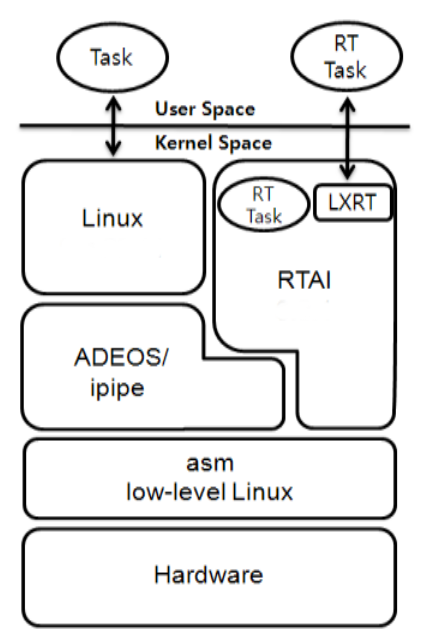
\includegraphics[scale=0.22]{files/rtai.png}
	\caption{Abordagem RTAI.}
	\label{fig:rtai}
\end{figure}

\begin{figure}[h]
	\centering
	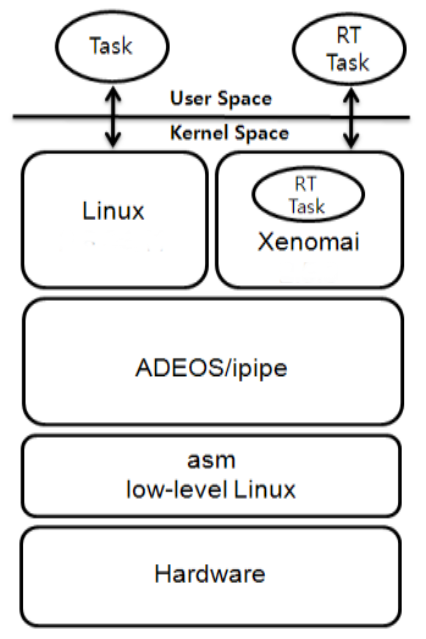
\includegraphics[scale=0.22]{files/xenomai.png}
	\caption{Abordagem Xenomai.}
	\label{fig:xenomai}
\end{figure}

Devido à diferença estrutural, RTAI tende a ser mais performático que o Xenomai em termos de desempenho se comparados os tempos de latência das interrupção, enquanto que Xenomai, com a sua estrutura simplificada, trata as interrupções com maior consistência \cite{Barbalace_rtai_xenomai}.

Ambos RTAI e Xenomai possuem comunidade de desenvolvedores bastante ativas e ambos são alternativas a implementação desse trabalho devido a compatibilidade com as outras ferramentas propostas, porém, apenas uma abordagem utilizando Xenomai será considerada. 

\begin{figure}[h]
	\centering
	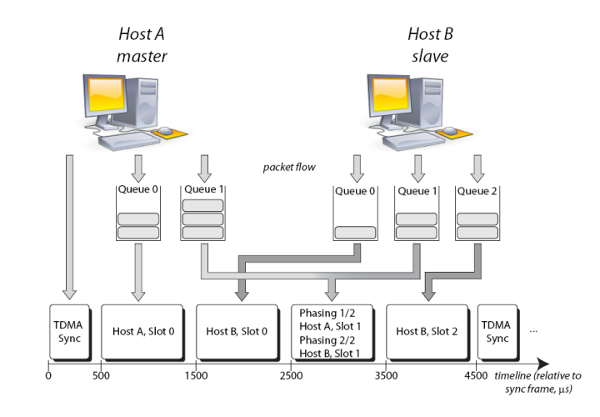
\includegraphics[scale=0.33]{files/rtnet_tdma.png}
	\caption{RTnet ciclo do TDMA.  \cite{rtnet_org}}
	\label{fig:rtnet_tdma}
\end{figure}

Quando uma estação \textit{slave} é conectada a rede, então, é iniciado um procedimento de sincronização com a estação \textit{master} repetido várias vezes, a fim de estimar o atraso médio de transmissão. O número de repetições depende da variância esperada das medições e deve ser escolhido de forma adequada.

Atualmente a abordagem RTnet suporta alguns dos principais dispositivos de rede, que são:
\begin{itemize}
	\item Intel 8255x EtherExpress Pro100
	\item Intel PRO/1000 (Gigabit Ethernet)
	\item DEC 21x4x Tulip
	\item RealTek RTL8139
	\item RealTek RTL8169 (Gigabit Ethernet)
	\item AMD PCnet32/PCnetPCI
	\item VIA Rhine
	\item NatSemi DP8381x
	\item MPC8xx (SCC and FEC Ethernet)
	\item MPC8260 (FCC Ethernet)
	\item MPC5200
	\item SMSC LAN91C111
\end{itemize}

\begin{figure}[h]
	\centering
	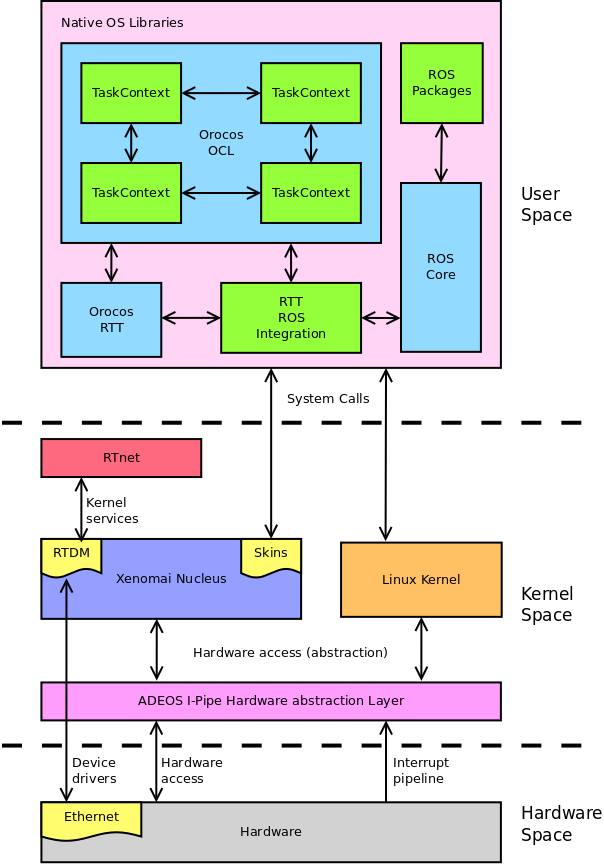
\includegraphics[scale=0.33]{files/VILMA_ENV_OVERVIEW.png}
	\caption{Visão geral da arquitetura proposta.}
	\label{fig:vilma_env_overview}
\end{figure}

RTnet é executado no espaço do \textit{kernel} Xenomai, ou seja, é parte do próprio \textit{kernel}, e fornece facilidades de rede para os aplicativos do usuário por meio de um conjunto de chamadas do sistema. Em outras palavras, o gerenciador da pilha é uma tarefa do \textit{kernel} de tempo real que manipula os pacotes de rede em nome do \textit{kernel} Xenomai, enviando e recebendo-os dos \textit{drivers} que comunicam diretamente com \textit{hardware}. Cada pacote de dados proveniente do espaço de usuário é então encaminhado ao gerenciador da pilha, que adiciona os cabeçalhos necessários, processa o encaminhamento e gerencia a fila de transmissão para cada interface de rede. Por outro lado, quando um pacote é recebido por uma interface de rede, uma interrupção assíncrona é desencadeada pelo dispositivo de \textit{hardware} para sinalizar a recepção de pacotes ou alguma condição de erro, então o ADEOS I-Pipe redireciona a interrupção para Xenomai que passa o controle ao \textit{driver} de tempo real. O pacote é copiado para à memoria e repassado para o gerenciador da pilha, que o entrega para a aplicação do usuário ou descarta o mesmo.

% -------------------- NEW SECTION -------------------- 
% -------------------- NEW SECTION -------------------- 
% -------------------- NEW SECTION -------------------- 

\section{Sistema Supervisor}\label{sec:supervisory_system}

O desenvolvimento de um sistema para controle supervisório é o propósito desde trabalho, o VilmaSpervisor, que realiza o gerenciamento e a coleta de informações dos outros componentes do Veículo. Assim sendo, deve-se fornecer aos demais pesquisadores do FEM-LMA meios para que possam instrumentar seus projetos com a o mínimo de modificação possível, possibilitando a supervisão dos sistemas de forma "transparente". além disso, o consumo de recursos do sistema deve ser o mínimo possível para não impactar na performance dos projetos.

O componente VilmaSupervisor também deve garantir a integridade dos componentes necessários à execução das tarefas de navegação autônoma, onde uma mensagem de \textit{heartbeat} será solicitada periodicamente a fim de garantir a presença e funcionamento adequado dos componentes presentes no sistema. Alem disso, VilmaSupervisor deve repassar as informações coletadas para um componente da camada superior, onde será apresentado ao administrador do sistema tais dados. O objetivo é, naturalmente, que o usuário possa dizer se um componente está se comportando corretamente ou não, sem ter qualquer conhecimento do supervisor.

\subsection{Especificações}\label{subsec:specifications}

O desenvolvimento do projeto VilmaSupervisor consiste de quatro partes. A primeira delas, a instrumentação dos demais projetos do Veículo autônomo VILMA. Esses componentes devem produzir informações que serão consumidas pelo sistema supervisório. Logo, as informações são tratadas e armazenadas em um componente denominado VilmaResources. Por fim, um outro componente, VilmaMonitor, vai ler estas informações armazenadas e repassá-las ao sistema de interface de usuário.

\subsubsection{Instrumentação}\label{subsec:instrumentation}

Vamos precisar fornecer aos pesquisadores do laboratério FEM-LMA com ferramentas que possam facilmente integrar o controle supervisório a seu projeto. Sendo assim, existem duas formas para realizar a instrumentação dos projetos desenvolvidos para o Veículo autônomo VILMA a integração com o sistema supervisório. Como pode ser visto na Figura \ref{fig:use_case_instrumentacao}.

\begin{itemize}
	\item Integração automática: herdando a classe VilmaTask como classe base;
	\item Integração manual: instanciando um objeto SupervisorComponent como membro da classe;
\end{itemize}

\begin{figure}[h]
	\centering
	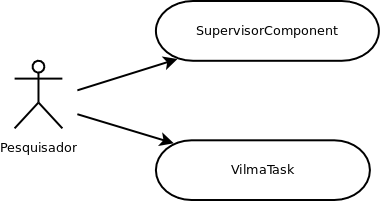
\includegraphics[scale=0.22]{files/USE_CASE_INSTRUMENTATION.png}
	\caption{Casos de uso da instrumentação.}
	\label{fig:use_case_instrumentacao}
\end{figure}

O primeiro método de integração consiste em uma classe chamada TaskVilma onde os pesquisadores devem utilizá-la como classe base para seus componentes, ao invés de utilizaram a classe primitiva de Orocos TaskContext. Uma vez que TaskVilma é uma classe derivada de TaskContext com a infraestrutura necessária para possibilitar a supervisão do Veículo VILMA, todos os métodos originais fornecidos por TaskContext também estão presentes em TaskVilma.

Ao utilizar TaskVilma, os desenvolvedores terão que implementar alguns métodos, ao invés dos métodos padrões de TaskContext, necessários para realizar os procedimentos de supervisão. A necessidade destas novas funções intermediárias será explicada em detalhas na subseção \ref{subsec:implementacao}. está é a única diferença quando se utiliza a classe TaskVilma, o que traz a capacidade de supervisão completa com um pequeno esforço do lado dos desenvolvedores.

O segundo método consiste em um novo componente, SupervisorComponent, onde é necessário criar a instancia de um objeto a um componente que não implemente a classe TaskVilma. Este objeto contém uma série de métodos que seráo necessários que precisam ser invocados no interior dos métodos padrões da classe TaskContext, a fim de adicionar supervisão.

No entanto, vamos também fornecer um objeto wrapper que fará a supervisão manual de uma tarefa mais simples. A classe TaskVilma será implementado utilizando a SupervisorComponent.

%Users that wish to customize which metrics and tests are done
%for their components will find the ComponentSupervisor fitting for
%their needs. If, on the other hand, they just want a quick way to add
%instrumentation to their code the use of PalTask is encouraged.

\subsection{Projeto de Software}\label{subsec:software_design}

We will now proceed to explain the OroSupervisor project pipeline,
i.e. the path the information follows, from the user?s component to
the Supervisor robot monitor passing through the OroSupervisor.
The classes, structures and communication objects that will be need
to be used will be also a part of this section. An Unified Modeling
Language ( UML ) representation of the pipeline can be seen in Figure
11. Keep in mind, this is not the full class diagram of the project. To
keep it simple, some details have been left out. Each scope of the
project will be better described later.
First, users will need to instrument their Orocos components using
one of the two methods explained in the Instrumentation subsection.

\subsubsection{VIS processos de software}\label{subsec:vis_processos_sw}

O componente VIS é constituído por dois processos de software. Sendo um baseado em processo \textit{event-driven} [], com a finalidade da coordenação das atividades entre os componentes sinalizando a troca de estados. E o outro baseado em processo periódico, \textit{periodic-tasks} [], para monitoramento da integridade dos componentes presentes na arquitetura do projeto VILMA.

O processo \textit{event-driven} é responsável pela execução de três tarefas: 
\begin{enumerate}
	\item Executar a sequência de mudança do modo operacional.
	\item Realizar o roteamento dos dados relevantes entre os componentes.
	\item Exibir as informações de estado do Veículo e seus componentes.
\end{enumerate}

O processo periódico é responsável por monitorar continuamente a integridade de todos os componentes durante a realização das tarefas. Aguardando o recebimento uma mensagem \textit{time-stamped} [], chamada de \textit{heartbeat}, em uma frequência predefinida para cada componente.

Se a frequência de chegada dos \textit{heartbeats} de um componente corresponde a um valor pré-definido, então, o VIS assume que este componente em particular está funcionando normalmente.

Caso o VIS não receba o \textit{heartbeat} de um componente por três amostras de tempo consecutivas, então o VIS assumirá que aquele componente em particular não está funcionando corretamente, assim, ele irá instruir todos os componentes a se moverem para o estado \textit{Standby}, para avaliação da possível falha.

O processo periódico do VIS precisa enviar uma mensagem de \textit{heartbeat} para o \textbf{Vehicle Safety Module} (VSM), para que o VSM possa monitorar a integridade operacional do VIS, caso as mensagens de \textit{heartbeat} do VIS não cheguem ao VSM, este deve instruir o sistema ao procedimento de emergência.

Para exemplificar este cenário, a frequência das mensagens de \textit{heartbeat} para todos componentes (exceto o VIS) será configurara para 1Hz. Essa seleção deve ser baseada considerando a distancia que o Veículo percorrerá a partir do momento que a falha de um componente seja detectada pelo VIS até o instante em que o Veículo estiver totalmente parado. Este deslocamento será chamado de distância \textit{fail-stop}.

Suponha a velocidade \textit{s} em \textit{km/h} e a distância de parada do Veículo \textit{d} em metros.

Com uma frequência de 1Hz para as mensagens de \textit{heartbeats}, o VIS conseguirá detectar uma falha em um componente após 1 segundo. Durante este 1 segundo, o Veículo terá percorrido uma distancia de \textit{1000s/3600} metros.	

Assumindo que o tempo necessário para que o VIS instrua o componente responsável pelos atuadores a pararem o Veículo seja desprezível, então a distancia \textit{fail-stop} será \textit{d + (1000s/3600)} metros.

Ainda como exemplo, assumindo \textit{s = 10km/h}, \textit{d = 4m} e \textit{(1000s/3600) = 2.8m}. Assim a distancia \textit{fail-stop} quando o Veículo estiver se movendo a velocidade de \textit{10km/h} será \textit{4+2.8 = 6.8} metros, em condições ideais.


\subsection{implementação}\label{subsec:implementation}

Since almost all of the code developed by PAL Robotics is programmed
in C++, our project will naturally be too. Also, is the same language
used in Orocos.
Besides all the custom tools developed by our company that are at
our service, we will also use the Boost C++ library.
Boost is a set of free C++ source libraries. They work well with the
C++ STL and are intended to be widely useful, and usable across a
broad spectrum of applications. The final goal is that Boost libraries are
suitable for eventual standardization. Ten Boost libraries are already
included in the C++ Standards Committee?s Library Technical Report
(TR1) and will be in the new C++0x Standard now being finalized.
C++0x will also include several more Boost libraries in addition to
those from TR1. More Boost libraries are proposed for TR2[1].

\subsubsection{VILMA::core::VariantType}\label{subsubsec:variant_type}

\subsubsection{VILMA::core::TaskVilma}\label{subsubsec:task_vilma}

\subsubsection{VILMA::VIS::HeartbeatType}\label{subsubsec:heartbeat_type}

\subsubsection{VILMA::VIS::Watchdog}\label{subsubsec:watchdog}

\subsubsection{VILMA::VIS::Supervisor}\label{subsubsec:supervisor}

\subsubsection{VILMA::VIS::Reporter}\label{subsubsec:reporter}

\subsubsection{Vilma Integrity System (VIS)}\label{subsubsec:vis}

% -------------------- NEW SECTION -------------------- 
% -------------------- NEW SECTION -------------------- 
% -------------------- NEW SECTION -------------------- 

\section{Testes e resultados}\label{sec:tests_results}

\subsection{Ambiente de testes}\label{subsubsec:tests_environment}

\subsection{Resultados obtidos}\label{subsubsec:results}

% -------------------- NEW SECTION -------------------- 
% -------------------- NEW SECTION -------------------- 
% -------------------- NEW SECTION -------------------- 

\section{Conclusões}\label{sec:conclusion}

Foi apresentada a proposta de projeto para a arquitetura do módulo de controle supervisório e sua proposta de implementação preliminar para o projeto VILMA a fim de atender o objetivo geral deste estudo, realizar operações autônomas em ambiente terrestre de forma segura.  

De acordo com esta arquitetura, o comportamento do Veículo é gerado pela da adoção de uma estrutura uniforme utilizando transições de estados genéricos para cada componente no Veículo. Esta estrutura representa um subconjunto comportamental dos componentes reconhecidos pelo VIS

Espera-se que a adoção desta arquitetura possa facilitar a síntese de estratégias para que o controle supervisório seja sofisticado através de técnicas de formalização para processos baseados em eventos. Uma vez que estratégias mais sofisticadas de controle supervisório podem melhorar o grau de autonomia do Veículo, representando portanto, um próximo passo para o desenvolvimento do Veículo autônomo VILMA.

também foi abordada uma arquitetura primária formada por um arcabouço tecnológico com foco em tornar o trabalho do grupo de pesquisa do projeto VILMA padronizado, priorizando a agilidade e a continuidade das pesquisas desenvolvidas no LMA e que atendesse aos requisitos que à aplicação necessita. 

A integração entre os sistemas de baixo nível (Linux, Xenomai, RTnet), possibilita à obtenção de resultados dentro do escopo dos sistemas críticos de tempo real distribuídos, essas tecnologias tem sido amplamente utilizadas e consolidadas nas industrias e grupos de pesquisa. 

Por fim a integração entre os sistemas para o desenvolvimento ágil no escopo das aplicações de usuário (ROS e OROCOS), baseada nas funcionalidades entre os fluxos de dados dos componentes dos \textit{frameworks} utilizados, reforça a ideia de agilidade e simplificação para o desenvolvimento das pesquisas.

Enquanto ROS possui bom suporte para a componentes distribuídos através da rede \textit{Ethernet}, OROCOS oferece suporte à tarefas de comunicação entre componentes que necessitem de garantias temporais. Isso combina o melhor dos dois mundos: o controle em tempo real de baixo nível é tratado por um conjunto de componentes OROCOS-RTT que controlam diretamente a troca de estados e modos de operação do Veículo, mas a comunicação entre os controladores é visível para toda a rede dos sistemas ROS.

Por fim, a integração torna os componentes OROCOS como sendo componentes ROS, sem que haja quebra nos requisitos de tempo real entre os componentes OROCOS-RTT. Permitindo que sejam utilizadas as diversas ferramentas desenvolvidas para ROS, como \textit{rviz} e \textit{rxplot}, para visualizar a comunicação entre os controladores.

% -------------------- NEW SECTION -------------------- 
% -------------------- NEW SECTION -------------------- 
% -------------------- NEW SECTION -------------------- 
\section{Próximos trabalhos}\label{sec:next_works}

Um vez definido o ponto de partida do conceito e componentes presentes na arquitetura do projeto VILMA e do sistema de controle supervisório, os próximos trabalhos estarão voltados para à especificação dos requisitos funcionais do VIS, consequentemente implementação do estudo apresentado, definição de testes para validação dos objetivos propostos e simulações da integração do VIS ao Veículo VILMA.

% -------------------- NEW SECTION -------------------- 
% -------------------- NEW SECTION -------------------- 
% -------------------- NEW SECTION -------------------- 

% use section* for acknowledgment
\section*{Acknowledgment}\label{sec:acknowledgment}

The authors would like to thank...

% trigger a \newpage just before the given reference
% number - used to balance the columns on the last page
% adjust value as needed - may need to be readjusted if
% the document is modified later
%\IEEEtriggeratref{8}
% The "triggered" command can be changed if desired:
%\IEEEtriggercmd{\enlargethispage{-5in}}

% references section

% -------------------- NEW SECTION -------------------- 
% -------------------- NEW SECTION -------------------- 
% -------------------- NEW SECTION -------------------- 
% \section{Referências}\label{sec:references}

% can use a bibliography generated by BibTeX as a .bbl file
% BibTeX documentation can be easily obtained at:
% http://www.ctan.org/tex-archive/biblio/bibtex/contrib/doc/
% The IEEEtran BibTeX style support page is at:
% http://www.michaelshell.org/tex/ieeetran/bibtex/
%\bibliographystyle{IEEEtran}
% argument is your BibTeX string definitions and bibliography database(s)
%\bibliography{IEEEabrv,../bib/paper}
%\bibliography{referencias}
% <OR> manually copy in the resultant .bbl file
% set second argument of \begin to the number of references
% (used to reserve space for the reference number labels box)
\begin{thebibliography}{1}
	\bibitem{IEEEhowto:kopka}
	H.~Kopka and P.~W. Daly, \emph{A Guide to \LaTeX}, 3rd~ed.\hskip 1em plus
	0.5em minus 0.4em\relax Harlow, England: Addison-Wesley, 1999.
\end{thebibliography}

% An example of a floating figure using the graphicx package.
% Note that \label must occur AFTER (or within) \caption.
% For figures, \caption should occur after the \includegraphics.
% Note that IEEEtran v1.7 and later has special internal code that
% is designed to preserve the operation of \label within \caption
% even when the captionsoff option is in effect. However, because
% of issues like this, it may be the safest practice to put all your
% \label just after \caption rather than within \caption{}.
%
% Reminder: the "draftcls" or "draftclsnofoot", not "draft", class
% option should be used if it is desired that the figures are to be
% displayed while in draft mode.
%
%\begin{figure}[!t]
%\centering
%\includegraphics[width=2.5in]{myfigure}
% where an .eps filename suffix will be assumed under latex, 
% and a .pdf suffix will be assumed for pdflatex; or what has been declared
% via \DeclareGraphicsExtensions.
%\caption{Simulation results for the network.}
%\label{fig_sim}
%\end{figure}

% Note that IEEE typically puts floats only at the top, even when this
% results in a large percentage of a column being occupied by floats.


% An example of a double column floating figure using two subfigures.
% (The subfig.sty package must be loaded for this to work.)
% The subfigure \label commands are set within each subfloat command,
% and the \label for the overall figure must come after \caption.
% \hfil is used as a separator to get equal spacing.
% Watch out that the combined width of all the subfigures on a 
% line do not exceed the text width or a line break will occur.
%
%\begin{figure*}[!t]
%\centering
%\subfloat[Case I]{\includegraphics[width=2.5in]{box}%
%\label{fig_first_case}}
%\hfil
%\subfloat[Case II]{\includegraphics[width=2.5in]{box}%
%\label{fig_second_case}}
%\caption{Simulation results for the network.}
%\label{fig_sim}
%\end{figure*}
%
% Note that often IEEE papers with subfigures do not employ subfigure
% captions (using the optional argument to \subfloat[]), but instead will
% reference/describe all of them (a), (b), etc., within the main caption.
% Be aware that for subfig.sty to generate the (a), (b), etc., subfigure
% labels, the optional argument to \subfloat must be present. If a
% subcaption is not desired, just leave its contents blank,
% e.g., \subfloat[].


% An example of a floating table. Note that, for IEEE style tables, the
% \caption command should come BEFORE the table and, given that table
% captions serve much like titles, are usually capitalized except for words
% such as a, an, and, as, at, but, by, for, in, nor, of, on, or, the, to
% and up, which are usually not capitalized unless they are the first or
% last word of the caption. Table text will default to \footnotesize as
% IEEE normally uses this smaller font for tables.
% The \label must come after \caption as always.
%
%\begin{table}[!t]
%% increase table row spacing, adjust to taste
%\renewcommand{\arraystretch}{1.3}
% if using array.sty, it might be a good idea to tweak the value of
% \extrarowheight as needed to properly center the text within the cells
%\caption{An Example of a Table}
%\label{table_example}
%\centering
%% Some packages, such as MDW tools, offer better commands for making tables
%% than the plain LaTeX2e tabular which is used here.
%\begin{tabular}{|c||c|}
%\hline
%One & Two\\
%\hline
%Three & Four\\
%\hline
%\end{tabular}
%\end{table}


% Note that the IEEE does not put floats in the very first column
% - or typically anywhere on the first page for that matter. Also,
% in-text middle ("here") positioning is typically not used, but it
% is allowed and encouraged for Computer Society conferences (but
% not Computer Society journals). Most IEEE journals/conferences use
% top floats exclusively. 
% Note that, LaTeX2e, unlike IEEE journals/conferences, places
% footnotes above bottom floats. This can be corrected via the
% \fnbelowfloat command of the stfloats package.
\end{document}